% arara: pdflatex
% arara: pdflatex
% arara: pdflatex

% options:
% thesis=B bachelor's thesis
% thesis=M master's thesis
% czech thesis in Czech language
% slovak thesis in Slovak language
% english thesis in English language
% hidelinks remove colour boxes around hyperlinks

\documentclass[thesis=B,czech]{FITthesis}[2012/06/26]

\usepackage[utf8]{inputenc} % LaTeX source encoded as UTF-8

\usepackage{graphicx} %graphics files inclusion
% \usepackage{amsmath} %advanced maths
% \usepackage{amssymb} %additional math symbols

\usepackage{dirtree} %directory tree visualisation

\usepackage[shortlabels]{enumitem}
\usepackage[font=footnotesize]{caption}
\usepackage{listings}
\usepackage{color, colortbl}

\definecolor{lightgray}{rgb}{.97,.97,.97}
\definecolor{darkgray}{rgb}{.4,.4,.4}
\definecolor{dkgreen}{rgb}{0,0.6,0}
\definecolor{azure}{rgb}{.014, .63, .6}
\definecolor{purple}{rgb}{.65, .12, .82}
\definecolor{lightgreen}{rgb}{0.9, 0.99, 0.9}
\definecolor{lightyellow}{rgb}{0.99, 0.97, 0.9}
\definecolor{lightred}{rgb}{0.99, 0.9, 0.9}

\lstdefinelanguage{JavaScript}{
	keywords={typeof, new, true, false, catch, function, return, null, catch, switch, var, if, in, while, do, else, case, break,class, export, boolean, throw, implements, import, this, const, async, await, for, from},
	keywordstyle=\color{blue}\bfseries,
	ndkeywords={expect, undo, toBe, _click, _clickWithCtrl, startMouseSelection, isSelected},
	ndkeywordstyle=\color{azure}\bfseries,
	identifierstyle=\color{black},
	sensitive=false,
	comment=[l]{//},
	morecomment=[s]{/*}{*/},
	commentstyle=\color{dkgreen}\ttfamily,
	stringstyle=\color{purple}\ttfamily,
	morestring=[b]',
	morestring=[b]`
}
\lstset{
	backgroundcolor=\color{lightgray},
	extendedchars=true,
	basicstyle=\footnotesize\ttfamily,
	showstringspaces=false,
	showspaces=false,
	numbers=left,
	numberstyle=\footnotesize,
	numbersep=9pt,
	tabsize=2,
	breaklines=true,
	showtabs=false,
	captionpos=b
}
\renewcommand{\lstlistingname}{Ukázka kódu}

% % list of acronyms
% \usepackage[acronym,nonumberlist,toc,numberedsection=autolabel]{glossaries}
% \iflanguage{czech}{\renewcommand*{\acronymname}{Seznam pou{\v z}it{\' y}ch zkratek}}{}
% \makeglossaries

\newcommand{\tg}{\mathop{\mathrm{tg}}} %cesky tangens
\newcommand{\cotg}{\mathop{\mathrm{cotg}}} %cesky cotangens

% % % % % % % % % % % % % % % % % % % % % % % % % % % % % % 
% ODTUD DAL VSE ZMENTE
% % % % % % % % % % % % % % % % % % % % % % % % % % % % % % 

\department{Obor Webové a softwarové inženýrství (BI-WSI), zaměření Softwarové inženýrství\\Katedra softwarového inženýrství}
\title{Webová aplikace pro online web scraping}
\authorGN{Jakub} %(křestní) jméno (jména) autora
\authorFN{Drahoš} %příjmení autora
\authorWithDegrees{Jakub Drahoš} %jméno autora včetně současných akademických titulů
\author{Jakub Drahoš} %jméno autora bez akademických titulů
\supervisor{Mgr. Martin Podloucký}
\acknowledgements{Doplňte, máte-li komu a za co děkovat. V~opačném případě úplně odstraňte tento příkaz.}
\abstractCS{Tato práce se zabývá vývojem nástroje umožňující web scraping. Cílí přede-vším na uživatele, kteří nedisponují znalostmi programování a tvorby webo-vých stránek. Původním záměrem byla tvorba webové aplikace, avšak ukázalo se, že takové řešení není svou složitostí adekvátní k danému problému. Z tohoto důvodu bylo nakonec řešení implementováno jako rozšíření do internetového prohlížeče Google Chrome. Software byl úspěšně navrhnut, realizován a otestován. Zároveň byla provedena analýza stávajících řešení, díky níž bylo možné najít nedostatky konkurenčních nástrojů (především pak složité ovládání) a nabídnout uživatelům aplikaci, jež těmito neduhy netrpí. Práce čtenáři nabídne také úvod do právní problematiky web scrapingu a shrnuje důležité poznatky z českého, evropského i kontinentálního práva na jednom místě.}
\abstractEN{Sem doplňte ekvivalent abstraktu Vaší práce v~angličtině.}
\placeForDeclarationOfAuthenticity{V~Praze}
\declarationOfAuthenticityOption{4} %volba Prohlášení (číslo 1-6)
\keywordsCS{web scraping, extrakce dat, aplikace, JavaScript, rozšíření prohlížeče Chrome, právní rozbor}
\keywordsEN{web scraping, data extraction, application, JavaScript, Chrome extension, legal analysis}

\begin{document}

% \newacronym{CVUT}{{\v C}VUT}{{\v C}esk{\' e} vysok{\' e} u{\v c}en{\' i} technick{\' e} v Praze}
% \newacronym{FIT}{FIT}{Fakulta informa{\v c}n{\' i}ch technologi{\' i}}

\begin{introduction}
	\vfill
	\section*{Cíle práce}
	Hlavním cílem této práce je návrh a tvorba softwaru, který bude umožňovat uživatelům extrahovat požadovaná data z~libovolné stránky v~reálném čase bez jakékoli nutné znalosti programování. Při specifikaci požadavků tohoto nástroje se přihlídne k~analýze stávajících řešení, jež je vedlejším cílem této práce. Druhým vedlejším cílem je poskytnout čtenáři úvod do právní problematiky web scrapingu a shrnout na jednom místě fakta, která máme k~dispozici.
	
	Neméně důležitou součást práce tvoří dodržení klasického vývojového cyklu softwarového projektu -- analýza, design, implementace a testování.
	
	Klíčovým aspektem aplikace je též \emph{přehlednost a jednoduchost uživatelského rozhraní} -- důraz bude kladen na intuitivní a rychlé ovládání.
	
	Naopak v~rozsahu této práce není tvorba web crawlera ani žádného jiného podobného mechanismu, jenž by systematicky a především \emph{automatizovaně} procházel danou oblast webu.
	
	\section*{Motivace}
	Věřím, že čím více informací se na internetu objevuje v~podobě webových stránek, tím více bude stoupat potřeba tyto informace určitým způsobem získávat a zpracovávat, například právě využitím web scrapingu. Dle mého názoru téměř kdokoli, kdo pracuje s~daty dostupnými z~internetu, může profitovat z~využití nějakého nástroje k~vytěžování dat a zvýšit tak svoji konkurenceschopnost.
	\newpage
	Tedy důvod k~vytvoření softwaru umožňující extrahovat data z~webových stránek je jasný. Ač podobných nástrojů existuje několik, jejich obsluha je~po-měrně složitá a je nutné strávit určitý čas, než se uživatel seznámí s~jejich fungováním a může je naplno využít. Právě tento aspekt se snaží aplikace vyvíjená v~rámci bakalářské práce eliminovat -- motivací je tak poskytnout uživatelům možnost jednoduše a rychle vytěžit požadovaná data bez zbytečného zdržování a dlouhého času stráveného seznamováním se s~nástrojem.
	
	To, čím je tato práce unikátní, je ale rozbor právního aspektu web scrapingu. V~žádném případě se nejedná o~hlubokou analýzu, která by byla očeká-vána od studenta právnické fakulty. Zároveň ale shrnuje podstatné poznatky a fakta z~dané oblasti na jednom místě. Velké množství textů dostupných na internetu, jenž se týkají tohoto tématu, totiž často začíná odstavcem ve stylu \uv{...nejsem právník a toto je jen můj názor...}, informace jsou velmi kusé a chybí jim nějaká ucelená struktura. To se práce snaží napravit a představuje tak vstupní bránu do této rozsáhlé problematiky. Zároveň může pomoct všem vývojářům, kteří tvoří software určený k~web scrapingu.
	
	\section*{Členění práce}
	Kapitola 1 je věnována analýze tématiky web scrapingu. První sekce shrnuje obecné informace, následuje pohled z~právní strany věci a nakonec analýza stávajících řešení problému. Kapitola 2 se zaměřuje na návrh aplikace -- specifikace požadavků, vymezení případů užití, architektura systému, návrh uživatel-ského rozhraní. Ve třetí kapitole je popsána realizace daného návrhu, výběr použitých technologií a odůvodnění rozhodnutí, která byla učiněna. Poslední kapitola je věnovaná testování celé aplikace. V~samotném závěru se pak zabý-vám vyhodnocením jednotlivých cílů zadaných výše.
	
	\section*{Poznámka}
	V~průběhu práce se objevily okolnosti (detailně jsou diskutovány v~kapitole \hyperref[sec:possible_solutions]{Realizace, sekce Diskuze možných řešení}), které mě donutily přehodnotit původní záměr tvorby webové aplikace na tvorbu rozšíření do internetového prohlížeče Google Chrome. To jsem bohužel nevěděl při formulaci a odevzdání zadání do systému závěrečných prací, tedy název této práce neodpovídá úplně přesně výslednému produktu. Nicméně všechny cíle zůstaly naprosto totožné.
\end{introduction}


% ================================================================================================


\chapter{Analýza}
V~této kapitole jsou představeny základní pojmy web scrapingu, jeho historie, způsoby, kterými extrakce dat z~internetových stránek nejčastěji probíhá a jak se takto získaná data dají využít. Hlavní částí této kapitoly je pak právní rešerše problematiky web scrapingu a analýza již existujících aplikací poskytujících uživatelské rozhraní pro vytěžování dat z~webových stránek.

% ------------------------------------------------------------------------------------------------

\section{Web scraping}
\uv{\textit{Web scraping (nebo také web harvesting, web data extraction) je softwarová technika zaměřená na extrakci informací z~webových stránek}}~\cite[překlad autora]{web_scraping_def}. Nejčastěji se v~tomto kontextu jedná o~automatizovaný proces strojového zpracování a získávání dat, nicméně může jít i~o~manuální extrakci zadanou uživatelem skrze nějaký software (jako je tomu právě v~našem případě).

Často se také v~souvislosti s~pojmem web scraping používá spojení \emph{web crawler} (nebo také \emph{bot, spider, spiderbot}). Jedná se o~automatizovaný software, který systematicky prochází danou oblast webu a během toho vytěžuje kýžená data.~\cite{web_crawler_def}

\subsection{Krátce z~historie}
Historie web scrapingu sahá k~samým počátkům internetu (World Wide Web, 1989). Prvním webovým robotem, který byl vyvinut na MIT k~měření velikosti webu, byl World Wide Web Wanderer (napsaný v~jazyce Perl) z~roku 1993.~\cite{web_wanderer}

O~něco později, v~roce 2000, se ve velkém začala používat webová API -- lidé mohli získávat čistá data přímo od serveru a scraping se tak stal o~hodně jednodušším. Dalším milníkem v~historii web scrapingu je rok 2004, kdy byla vydána knihovna pro parsování HTML a XML dokumentů Beautiful Soup pro programovací jazyk Python. Ta je do dnes považována za nejsofistikovanější a nejpokročilejší knihovnu pro web scraping. Za zmínku stojí určitě i~rok 2006, kdy je datován příchod vizuálního web scrapingu (\label{def:visual_web_scraping}\emph{visual web scraping}), tedy techniky, kdy uživatel skrze rozhraní aplikace označí klikáním myši, z~kterých oblastí webové stránky chce extrahovat data. Tímto se otevřely dveře web scrapingu pro všechny.~\cite{web_scraping_history}

\subsection{Techniky}
Technik, jak z~webové stránky získat data existuje mnoho, podívejme se alespoň na některé z~nich:
\begin{itemize}
	\item vyhledávání na základě textové shody -- např. pomocí UNIX nástroje grep nebo regulárních výrazů
	\item HTML parsování -- základní a stále ještě nejpoužívanější technika extrakce dat; informace jednoduše získáváme z~HTML elementů, popř. pomocí tříd nebo id
	\item počítačové vidění, strojové učení, zapojení umělé inteligence -- snaha napodobit způsob, jakým vidí a zpracovává webovou stránku člověk; podobný přístup zkouší např. projekt Diffbot~\cite{computer_vision}
	\item vizuální web scraping -- jak již bylo zmíněno výše, požadovaná data se musí ručně naklikat skrze rozhraní nějaké aplikace (značně to však usnadňuje např. hledání podobných prvků na základě prvních pár kliknutí)
	\item manuální vyhledávání a stahování dat (někdy nazývané také \emph{copy-paste})
\end{itemize}

\subsection{Využití web scrapingu}
Podob pro uplatnění scrapování dat z~webu je nespočet, a to obzvlášť v~dnešní době, kdy se dle~\cite{data_size} velikost všech dat na celém internetu pohybuje v~řádech Zettabajtů ($1024^{7}$ B). Mezi ty hlavní patří:
\begin{itemize}
	\item získání kontaktních informací (např. e-mail) pro marketingové účely
	\item indexování webových stránek, které však využívá hlavně web crawling (jako příklad můžeme uvést známý GoogleBot~\cite{google_bot})
	\item data mining -- proces hledání vzorců ve velkých datových setech~\cite{data_mining}
	\item monitorování různých proměnných (např. sledování cen nebo hodnocení produktů)
	\item recyklace již někdy použitých dat za účelem vytváření \uv{nového} obsahu
	\item analýza a zpracování dat k~výzkumným účelům
\end{itemize}

% ------------------------------------------------------------------------------------------------

\section{Právní aspekt}
\label{sec:pravni_aspekt}
Podrobná právní analýza celé problematiky web scrapingu by vydala na samostatnou diplomovou práci, a tak se pokusím pouze shrnout základní body, představit hlavní právní pojmy a poskytnout čtenáři alespoň náhled do této oblasti. 

Při získávání dat z~internetových stránek může nastat hned několik komplikací z~právního hlediska, na které by se autor takového softwaru měl připravit. Následuje stručný souhrn informací, kterým se podrobně věnují jednotlivé části celé této sekce.

Obsah může být chráněn autorským zákonem, pokud nabývá určitých rysů -- zejména se musí jednat o~výsledek tvůrčí činnosti autora. Zároveň pod tuto oblast mohou spadat věci jako je obyčejná databáze, způsob, jakým jsou určitá data rozvrstvena a uspořádána na stránce nebo třeba rozpis fotbalových utkání. Další kategorie, do kterých data mohou spadat, jsou osobní údaje a projevy osobní povahy. Při jejich zpracování je nutné postupovat přesně podle stanovených pravidel v~příslušných zákonech a právních úpravách. A~i~když data nejsou chráněna žádným zvláštním zákonem, stále je nutné řídit se smluv-ními podmínkami, které se mohou vztahovat na jakýkoliv obsah.

Tím nejkritičtějším místem každého web scrapingu je ale způsob využití samotných dat. Ve směs je možné říci, že pokud používám data čistě pro svoji osobní/domácí potřebu, pro věděcké nebo pedagogické účely (kde má ale každé užití své podstatné náležitosti) a bez účelu dosažení hospodářského prospěchu, s~největší pravděpodobností se nedopustím žádného protiprávního jednání. Vždy je ale tím nejbezpečnějším řešením kontaktovat provozovatele dané stránky a na detailech se dohodnout.

Nutno také podotknout, že celá tato oblast je relativně nová a zatím neexistuje jednotný právní precedent\footnote{Kontinentální právo (na rozdíl od anglosaského) nezná precedenty (tj. všeobecně závazná soudní rozhodnutí), resp. nepovažuje je právě za závazné. Na druhou stranu by soudy měly ve stejných případech postupovat stejně. Proto si zde dovolím tento výraz použít.}, podle kterého by se soudy mohli při posuzování jednotlivých případů řídit. Proto také můžeme nabýt pocitu, že i~když se jedná o~často velmi podobné případy, výsledky soudních sporů jsou diametrálně odlišné. To se ale může změnit s~případem \emph{hiQ v. LinkedIn}, který je pravděpodobně tím největším milníkem v~právní historii web scrapingu -- pokud se výsledek ještě zvrátí ve prospěch společnosti LinkedIn, mohlo by to znamenat velké omezení otevřeného přístupu k~informacím pro všechny.

\subsection{Základní pojmy}
\paragraph{Terms of Service} (někdy také \textit{Terms of Use}, \textit{Terms and Conditions}) je soubor pravidel sepsaný provozovatelem služby a říká, jak se uživatel smí chovat při užívání dané služby (v~kontextu této práce se jedná o~webové stránky) a co naopak dělat nesmí.

\paragraph{Browsewrap} je jeden ze způsobů dohody mezi dvěma stranami kontraktu. Není nutná žádná přímá interakce s~uživatelem, ať už jde o~souhlas či nesouhlas. Místo toho je na webové stránce (nejčastěji v~dolní části) umístěna krátká zpráva informující, že pouhým procházením daného webu souhlasí s~podmínkami používání (Terms of Service). Ty jsou umístěny na samostatné stránce, na kterou vede odkaz, jenž je součástí této zprávy. U~tohoto způsobu je těžké posoudit, zdali je tu jasný projev vůle, a tak je jeho vymahatelnost sporná a liší se případ od případu.~\cite{browse_wrap}

\paragraph{Clickwrap}\label{def:clickwrap} je oproti browse-wrap daleko lépe vymahatelný, neboť je uživa-tel nucen přímo vyjádřit souhlas či nesouhlas (kliknutím na tlačítko nebo zaškrtnutím políčka) se všemi uvedenými podmínkami, a to \emph{před} použitím dané služby. Tím je zde jasně určen projev vůle. Podmínky jsou stejně jako v~případě browsewrap často umístěny na samostatné stránce a je k~nim uveden pouze odkaz, i~když někdy je k~dispozici i~celé jejich znění. Jedná se o~tzv. \emph{ber nebo nech být} smlouvu -- \uv{\emph{Ber nebo nech být smlouva, také nazývána adhezní smlouva, říká, že smluvní podmínky nemůžou být vyjednávány.}}~\cite[překlad autora]{take_it_or_leave_it}.~\cite{click_wrap}

\subsection{Odpovědnost v~případě protiprávního jednání}
Ve chvíli, kdy se uživatel dopustí protiprávního jednání při využívání určitého nástroje, odpovědnost jednoznačně spočívá na něm, nikoliv na tvůrci aplikace. Zároveň je třeba upozornit, že autor softwaru odpovídá v~situaci, kdy je software primárně určen k~protiprávnímu jednání. Lze tedy jen doporučit, aby byl uživatel prokazatelně seznámen s~odpovědností za užívání softwaru v~souladu s~právem.~\cite{rozhovor}

\subsection{Obsah na webových stránkách a jeho možné využití}
Dle~\cite{rozhovor} může být obsah chráněn zejména jako:
\begin{itemize}
	\item projev osobní povahy
	\begin{itemize}
		\item zde lze připomenout z~občanského zákoníku -- \uv{\textit{Nikdo nesmí zasá-hnout do soukromí jiného, nemá-li k~tomu zákonný důvod. Zejména nelze bez svolení člověka narušit jeho soukromé prostory, sledovat jeho soukromý život nebo pořizovat o~tom zvukový nebo obrazový záznam, využívat takové či jiné záznamy pořízené o~soukromém životě člověka třetí osobou, nebo takové záznamy o~jeho soukromém životě šířit. Ve stejném rozsahu jsou chráněny i~soukromé písemnosti osobní povahy.}}~\cite[\S~86]{obcansky_zakon}
		\item do této kategorie můžou spadat třeba i~komentáře uživatelů na internetovém fóru
	\end{itemize}
	\newpage
	\item autorské dílo (včetně databáze, viz níže); z~autorského zákona lze zmínit:
	\begin{itemize}
		\item volné užití -- \uv{\textit{Za užití díla podle tohoto zákona se nepovažuje užití pro osobní potřebu fyzické osoby, jehož účelem není dosažení pří-mého nebo nepřímého hospodářského nebo obchodního prospěchu, nestanoví-li tento zákon jinak.}}~\cite[\S~30 odst.~1]{autorsky_zakon}
		\item citaci -- \uv{\textit{Do práva autorského nezasahuje ten, kdo
		\begin{enumerate}[a)]
			\item užije v~odůvodněné míře výňatky ze zveřejněných děl jiných autorů ve svém díle,
			\item užije výňatky z~díla nebo drobná celá díla pro účely kritiky nebo recenze vztahující se k~takovému dílu, vědecké či odborné tvorby a takové užití bude v~souladu s~poctivými zvyklostmi a v~rozsahu vyžadovaném konkrétním účelem,
			\item užije dílo při vyučování pro ilustrační účel nebo při vědeckém výzkumu, jejichž účelem není dosažení přímého nebo nepřímého hospodářského nebo obchodního prospěchu, a nepřesáhne rozsah odpovídající sledovanému účelu;
		\end{enumerate}
		vždy je však nutno uvést, je-li to možné, jméno autora, nejde-li o~dílo anonymní, nebo jméno osoby, pod jejímž jménem se dílo uvádí na veřejnost, a dále název díla a pramen.}}~\cite[\S~31 odst.~1]{autorsky_zakon}
	\end{itemize}
	\item osobní údaje (čl.~2 GDPR)
\end{itemize}

Je tedy možné shrnout, že použití pro osobní účely (resp. domácí činnosti) je v zásadě neomezené. Za vyzdvižení však stojí věta z~odstavce o~volném užití: \uv{\dots jehož účelem není dosažení přímého nebo \textit{nepřímého} hospodářského nebo obchodního prospěchu~\dots} -- když použiji získaná data na svém osobním blogu, kde ale mám určitou formu výdělku třeba v~podobě reklamy, mohu se již dopouštět protiprávního jednání.

Důležité je dát si velký pozor také při zpracování a využití osobních údajů, které upravuje čl.~2 GDPR -- toto téma by samo vydalo na několik desítek stránek, a tak se jím v~této práci nebudu zabývat a je zde zmíněno jen pro úplnost.

V~neposlední řadě je třeba poznamenat, že při vytěžování webu není podstatné, jakým způsobem k získání obsahu došlo (zdali prostřednictvím automatizovaného nebo manuálního postupu)\footnote{Otázkou je, jestli by bylo vůbec vymahatelné, pokud by měla stránka přímo ve svých Terms of Service uvedeno, že si nepřeje automatizované procházení, nehledě na to, jestli zároveň probíhá extrakce dat či nikoliv. Taková podmínka by mohla být brána jako neadekvátní a nepřiměřená.}. Důležité je, jestli tak činím \emph{v~souladu s~běžným, očekávaným a přiměřeným použitím} -- je tak nutné dát si pozor na detaily automatizovaného procházení, např. omezit počet požadavků na server, aby odpovídal běžnému použití lidským uživatelem\footnote{Tedy pokud je nějaký software schopný projít celou doménu během pár vteřin, je to náznak, že nemusí respektovat výše uvedené podmínky.}. Rozhodně lze ale doporučit provádět scraping webových stránek se souhlasem jejich provozovatele (poskytovatele), a to dle právního režimu dat a dané jurisdikce (situace u~nás je jiná než třeba v~USA).~\cite{rozhovor}

\subsection{Obsah chráněný autorským zákonem}
Autorské právo chrání na internetu různý obsah, zejména budou chráněny různé články, obrázky, videa atd. Vždy však bude muset naplňovat znaky autorského díla, tj. bude muset být \uv{\textit{\dots jedinečným výsledkem tvůrčí činnosti autora a být vyjádřen v~jakékoli objektivně vnímatelné podobě včetně podoby elektronické, trvale nebo dočasně, bez ohledu na jeho rozsah, účel nebo vý-znam\dots}}~\cite[\S~2 odst.~1]{autorsky_zakon}.

Taková kritéria však může splňovat i~obsah, který by se na první pohled vůbec nemusel zdát chráněný autorským zákonem -- jako příklad může posloužit celkové rozvržení stránky (neboli \textit{layout}), které ponese určitý prvek originality a bude na první pohled asociovatelné s~danou webovou stránkou.

Naopak výše zmíněnou definici určitě nesplňují různá počítačem generovaná data, tedy například logy chráněné autorským zákonem nebudou.

\subsection{Web scraping a zvláštní práva pořizovatele databáze}
Dle~\cite{rozhovor} žádný zvláštní zákon věnující se výslovně vytěžování webových stránek neexistuje. Z~naší právní úpravy je tomu nejblíže úprava zvláštního práva pořizovatele databáze (hlava III autorského zákona), která definuje, co to je databáze -- \uv{\textit{Databází je pro účely tohoto zákona soubor nezávislých děl, údajů nebo jiných prvků, systematicky nebo metodicky uspořádaných a individuálně přístupných elektronickými nebo jinými prostředky, bez ohledu na formu jejich vyjádření.}}~\cite[\S~88]{autorsky_zakon}. Za nezávislé se v~tomto kontextu považují prvky, \uv{\textit{které lze od sebe oddělit, aniž by tím byl dotčen jejich informační, literární, umělecký, hudební nebo jiný obsah}}~\cite{polcak}.

\uv{\textit{Tato právní úprava byla do autorského zákona převzata ze Směrnice Evropského parlamentu a Rady EU 96/9/ES, o~právní ochraně databází}}~\cite{ikaros}, a tak můžeme informace čerpané z~této sekce vztahovat nejen na Českou Republiku, ale na jakoukoli zemi Evropské Unie.

Dále jsou upraveny některé způsoby užití databáze v souladu s~autorským zákonem:
\begin{itemize}
	\item Omezení zvláštního práva pořizovatele databáze -- \uv{\textit{Do práva pořizo-vatele databáze, která byla zpřístupněna jakýmkoli způsobem veřejnosti, nezasahuje oprávněný uživatel, který vytěžuje nebo zužitkovává kvalitativně nebo kvantitativně nepodstatné části obsahu databáze nebo její části, a to k~jakémukoli účelu, za podmínky, že tento uživatel databázi užívá běžně a přiměřeně, nikoli systematicky či opakovaně, a bez újmy oprávněných zájmů pořizovatele databáze, a že nezpůsobuje újmu autorovi ani nositeli práv souvisejících s~právem autorským k~dílům nebo jiným předmětům ochrany obsaženým v~databázi.}}~\cite[\S~91]{autorsky_zakon}
	\item Bezúplatné zákonné licence -- \uv{\textit{Do práva pořizovatele jím zpřístupněné databáze též nezasahuje oprávněný uživatel, který vytěžuje nebo zužitko-vává podstatnou část obsahu databáze
		\begin{enumerate}[a)]
			\item pro svou osobní potřebu; ustanovení \S~30 odst. 3 zůstává nedotčeno,
			\item pro účely vědecké nebo vyučovací, uvede-li pramen, v~rozsahu odů-vodněném sledovaným nevýdělečným účelem, a
			\item pro účely veřejné bezpečnosti nebo správního či soudního řízení.
	\end{enumerate}}}~\cite[\S~92]{autorsky_zakon}
\end{itemize}

Tedy pokud využívám databázi čistě pro osobní potřebu či pro věděcké nebo vyučovací účely, kdy uvedu zdroj, je vše v~pořádku. Taktéž pokud využí-vám pouze nepodstatnou část obsahu databáze, a pokud tak dělám v~souladu s~běžným, očekávaným a přiměřeným použitím, nikoliv systematicky a opakovaně, je v~pořádku využití dokonce k~jakémukoliv účelu. Důležité je zde ale spojení \textit{oprávněný uživatel} -- v~každém případě musím mít k~datům autorizovaný přístup.

\subsection{Důležité soudní případy v~Evropě}
Rozbor jednotlivých soudních případů je velice důležitý, neboť právě podle nich se mohou soudy řídit při posuzování nových žalob a soudních rozepří. Stejně tak se o~ně mohou opírat žalobci i~obhájci a pro širokou veřejnost může být více předvídatelné, jak by se obdobné problémy mohly řešit v~budoucnu. Mezi nejvýznamnější rozhodnutí na půdě Soudního dvora Evropské unie patří:

\paragraph{C-444/02} kdy společnost Fixtures Marketing Limited (dále jen \uv{Fixtures}) žalovala společnost Organismos Prognostikon Agonon Podosfairou AE (dále jen \uv{OPAP}) kvůli opakovanému vytěžování rozpisů ligových soutěží ve fotbale v~Anglii (které vytvářela, sestavovala a zveřejňovala společnost Fixtures) a jejich následnému užití na webových stránkách společnosti OPAP.~\cite{C-444/02_1}

Výsledkem jednání bylo, že i~\emph{rozpis fotbalových utkání je databází} ve smyslu čl.~1 odst.~2 směrnice 96/9 a jako takový může být předmětem ochrany, kdy pořizovatel databáze má právo zabránit vytěžování nebo zužitkování dat. (ačkoliv u~společnosti Fixtures nebyl prokázán podstatný vklad, jenž by mohl odůvodnit poskytnutí ochrany).~\cite{C-444/02_2}

\paragraph{C‑30/14} kdy společnost Ryanair Ltd. žalovala společnost PR Aviation BV kvůli automatizovanému sběru dat o~cenách, letech a letových řádech, jež byly volně přístupné spotřebitelům z~webových stránek Ryanair Ltd. K~přístupu musel uživatel potvrdit souhlas (viz \hyperref[def:clickwrap]{sekce 1.2.1, definice pojmu clickwrap}) se všeobecnými podmínkami, ve kterých byl mimo jiné výslovně zakázán způsob, jakým data využívala PR Aviation BV. Tyto data pak společnost PR Aviation BV používala ke srovnávání cen na svém vlastním portálu.~\cite{C-30/14}

Soudní dvůr rozhodl ve prospěch Ryanair -- \emph{jestliže se autor databáze, která není chráněna autorským zákonem nebo právem pořizovatele, rozhodne poskytnout souhlas s~jejím využitím, nic mu nebrání ve stanovení smluvních podmínek}, jež by omezily používání databáze ze strany třetích osob, aniž by přitom bylo dotčeno použitelné vnitrostátní právo.~\cite{C-30/14}

\subsection{Důležité soudní případy ve Spojených státech}
Úprava v USA je postavena na jiné právní úpravě, a závěry tak nejsou automaticky přenositelné do našeho práva (což ovšem nevylučuje možnost použití těchto rozhodnutí pro účely argumentace). Představíme si dva nejdůležitější případy v~právní historii web scrapingu, se kterými mimo jiné vyvstávají otázky jako \uv{Komu doopravdy patří data uživatelů na internetu?} a \uv{Kdo má rozhodovat o~přístupu k~veřejným datům, jestli o~tom vůbec má někdo rozhodovat?}.

\paragraph{hiQ v. LinkedIn} kdy analytická společnost hiQ automatizovaně extrahovala veřejně dostupná (bez nutnosti registrace účtu) data z~profilů uživatelů sítě LinkedIn. Ta společnosti hiQ zaslala tzv. \textit{cease and desist letter} a požado-vala okamžité ukončení činnosti ze strany hiQ pod pohrůžkou porušení CFAA. \cite{hiq_linkedin_1}

K~dispozici je zatím pouze předběžné opatření ve prospěch hiQ, které říká, že \textit{nelze zabránit přístupu k~veřejně dostupným informacím} -- k~porušení CFAA (jako neoprávněný přístup) by došlo pouze v~případě obejití systému autentizace. Ze strany společnosti LinkedIn padl argument, že automatizovaný přístup k~veřejným datům není to samé jako normální \uv{osobní} užití, stejně jako je odlišné dlouhodobé sledování osoby přes GPS zařízení od letmého potkávání~\cite{linkedin_arg}. hiQ mimo jiné argumentoval i~tím, že sociální sítě jsou novodobá veřejná fóra (místa pro veřejné projevy, zejména politického charak-teru~\cite{public_forum}) a rozhodování o~udělení přístupu k~nim (ať už ze strany státu či soukromé společnosti) je porušením svobody slova a vyjadřování, a tím i~samotné ústavy státu Kalifornie.~\cite{hiq_linkedin_2}

\paragraph{Facebook v. Power Venture (Vachani)} kdy společnost Power Venture (CEO Steven Suraj Vachani), jež umožňovala agregovat různé sociální sítě a používat všechny jejich klíčové funkce z~jednoho místa, byla žalována sociální sítí Facebook kvůli neoprávněnému vytěžování profilů a zasílání e-mailů uživa-telům, které úmyslně vypadaly jako odeslané společností Facebook (údajné porušení CFAA, CAN-SPAM a California Penal Code, sekce 502). Facebook zaslal Power Venture \textit{cease and desist letter} a snažil se zamezit přístupu k~datům pomocí blokování IP adres. Power Venture přesto pokračoval ve své činnosti.~\cite{facebook_venture_1}

Soud rozhodl ve prospěch společnosti Facebook -- jednání Power Venture bylo v~rozporu se zákonem. Jako hlavní argument posloužil fakt, že Power Venture pokračoval ve svém jednání i~po explicitním odejmutí oprávnění přístupu k~datům společnosti Facebook. Zde je ale vhodné uvést, že Power Venture \emph{přistupoval k~profilům uživatelů pouze s~jejich vlastním souhlasem}, ač bez souhlasu Facebooku.~\cite{facebook_venture_2}

% ------------------------------------------------------------------------------------------------

\newpage
\section{Analýza konkurenčních nástrojů}
První skupinou, na kterou můžeme při hledání na internetu narazit, jsou společnosti, které nabízejí zákazníkům kompletní péči v~rámci extrakce dat. Cílí především na velké korporace, jimž postaví scrapovací nástroj přesně na míru, který poté také hostují a spravují. Zákazník tedy dostane data a o~nic víc se již nemusí starat. Jako příklad lze jmenovat třeba ContentGrabber~\cite{content_grabber}, Mozenda~\cite{mozenda} a další.

Pro tuto práci mnohem relevantnější kategorií je konkurenční nabídka nástrojů poskytujících uživatelům rozhraní k~web scrapingu. Zaměřím se pouze na takové nástroje, které nevyžadují jakoukoli znalost programování -- tedy žádné knihovny, API a nástroje pro budování vlastních scraperů.

Mezi ty největší představitele patří ParseHub~\cite{parsehub}, Octoparse~\cite{octoparse}, WebScraper~\cite{webscraper}, Dexi.io~\cite{dexio} a Data Scraper~\cite{data_scraper}. Čtyři ze zmíněných nástrojů jsou volně dostupné (které mají však velmi omezenou funkcionalitu a pokročilejší operace se odemknou až s~určitým platebním plánem -- tzv. freemium model) a jeden poskytuje bezplatně pouze 7denní zkušební verzi.

Předtím, než bude možné jednotlivé nástroje porovnávat, je nutné určit kritéria, podle kterých lze hodnotit kvalitu daného nástroje. Především půjde o~jednoduchost používání, celkovou přehlednost a rychlost, se kterou se uživa-tel dostane k~požadovaným datům. Důležitý je také způsob výběru dat, mož-nosti exportu získaných dat, jak aplikace sama dokáže uživatele seznámit s~používáním a také, v~jaké formě se nástroj vůbec používá a čím se od ostatních odlišuje (ať už v~pozitivním či negativním smyslu). 

Poj\v{d}me se tedy na některé nástroje podívat blíže:

\begin{figure}
	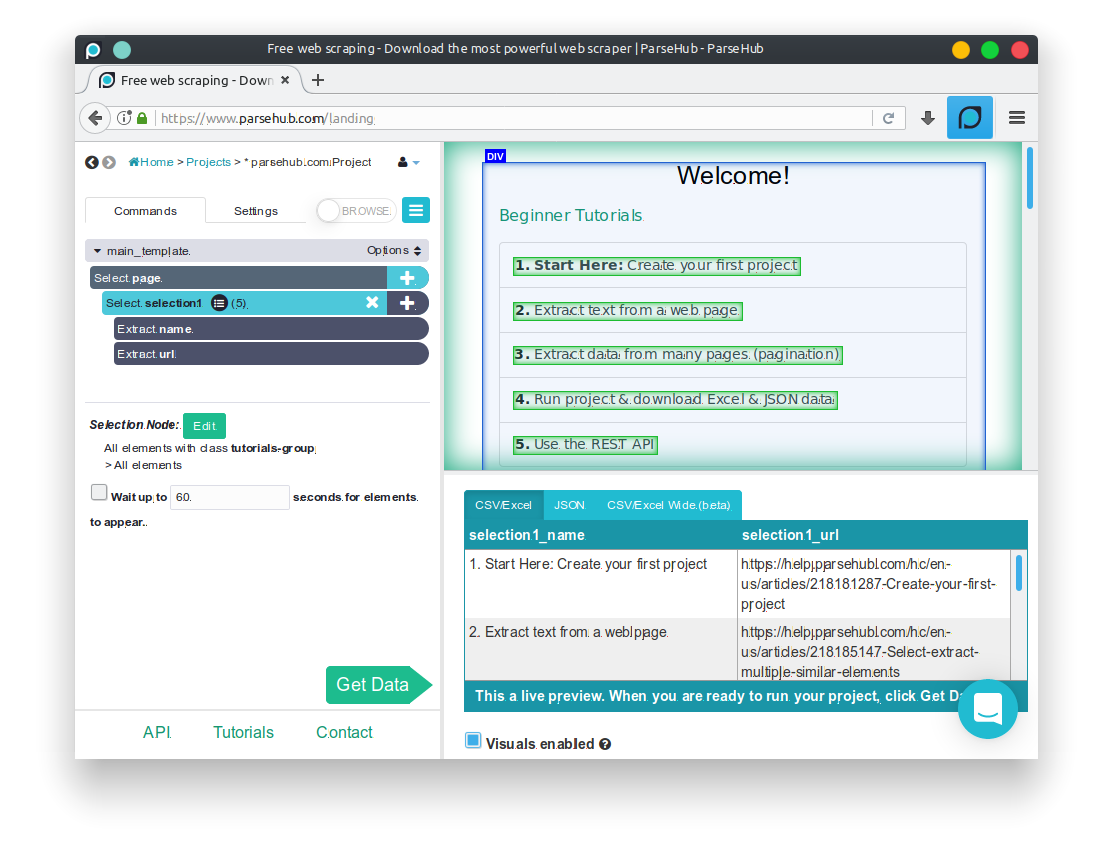
\includegraphics[width=\linewidth]{images/ParseHub.png}
	\caption[Desktopová aplikace ParseHub]{Desktopová aplikace ParseHub~\cite[snímek pořídil autor]{parsehub}}
	\label{fig:parseHub}
\end{figure}
\subsection{ParseHub}
\textbf{Výhody:}
\begin{itemize}
	\item výběr dat jak pomocí klikání (inteligentní hledání vzorců/podobností na základě prvních dvou kliknutí), tak pomocí XPath, regulárních výrazů nebo CSS selektorů
	\item aplikace obsahuje interaktivní tutoriál, který na jednoduchých příkladech ukáže, jak s~nástrojem zacházet
	\item možnost získání dat různými formami -- přes API, jako CSV/XLS, do GoogleSheets nebo do Tableau
	\item různé módy kliknutí (výběr, relativní výběr, kliknutí), zooming in/out na HTML elementy -- když se uživatel netrefí (nebo ani trefit nemůže) přesně na požadovaný prvek, lze na něj lehce přejít pomocí této funkce
	\item automatická rotace IP adresy (tedy nedochází k~blokování ze strany serveru)
\end{itemize}
\textbf{Nevýhody:}
\begin{itemize}
	\item nutnost stažení aplikace (ale je zde podpora pro Windows, Linux i~Mac)
	\item aplikace je celkově těžkopádná, nemá moc přívětivé uživatelské rozhraní, ovládání působí nepřehledně a přehlceně -- na uživatele se vyvalí hodně informací a možností najednou
\end{itemize}

\subsection{Octoparse}
\textbf{Výhody:}
\begin{itemize}
	\item výběr dat jak pomocí klikání (inteligentní hledání vzorců/podobností na základě prvních dvou kliknutí), tak pomocí XPath nebo regulárních výrazů
	\item nástroj obsahuje hotové šablony, které mohou velmi urychlit práci
	\item pestrá paleta možností (branch judgment, tvoření smyček apod.) -- dá se vytvořit téměř jakákoli logika procházení webu a extrakce dat
	\item lehký způsob, jak scrapování automatizovat
	\item možnost řídit tasky přes API (a získávat tak data taktéž přes API); data jdou nahrát rovnou i~do lokální databáze
\end{itemize}
\textbf{Nevýhody:}
\begin{itemize}
	\item nutnost stažení aplikace (která je navíc pouze pro Windows)
	\item těžkopádné a pomalé ovládání, neintuitivní rozhraní
	\item tutoriál je v~podstatě nic neříkající
	\item připravených šablon je jenom pár a jsou velmi konkrétní
\end{itemize}
\begin{figure}[h]
	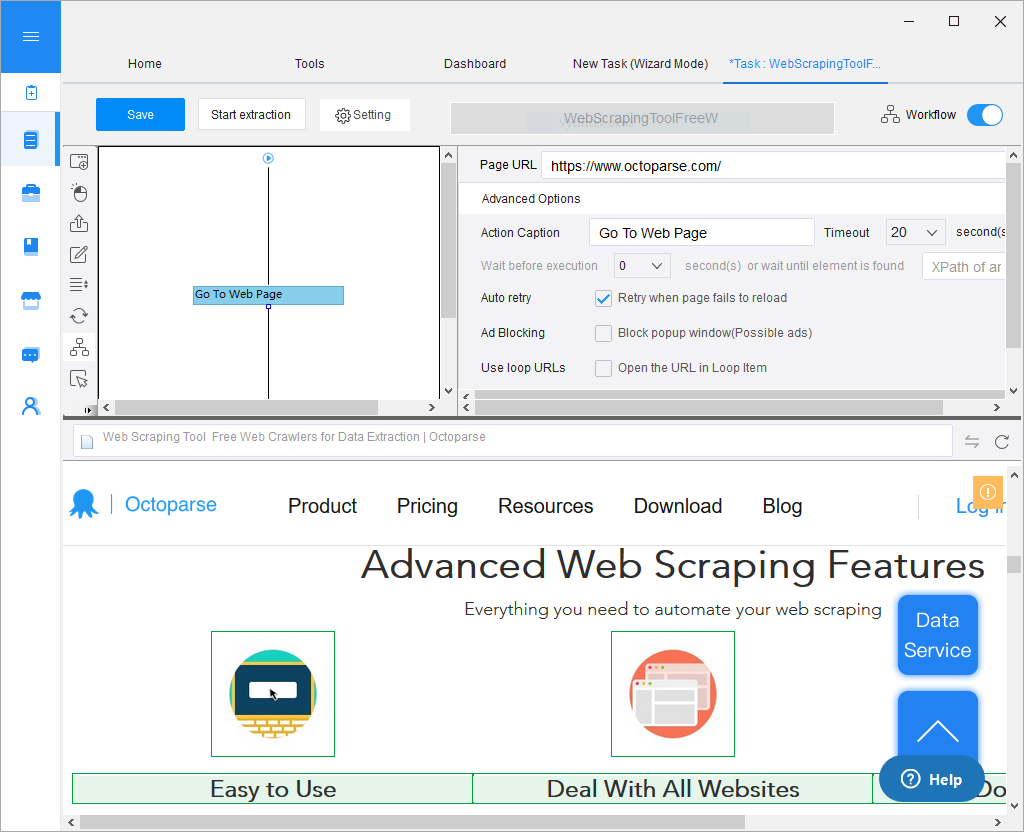
\includegraphics[width=\linewidth]{images/Octoparse.png}
	\caption[Desktopová aplikace Octoparse]{Desktopová aplikace Octoparse~\cite[snímek pořídil autor]{octoparse}}
	\label{fig:octoparse}
\end{figure}

\newpage
\subsection{WebScaper}
\begin{figure}
	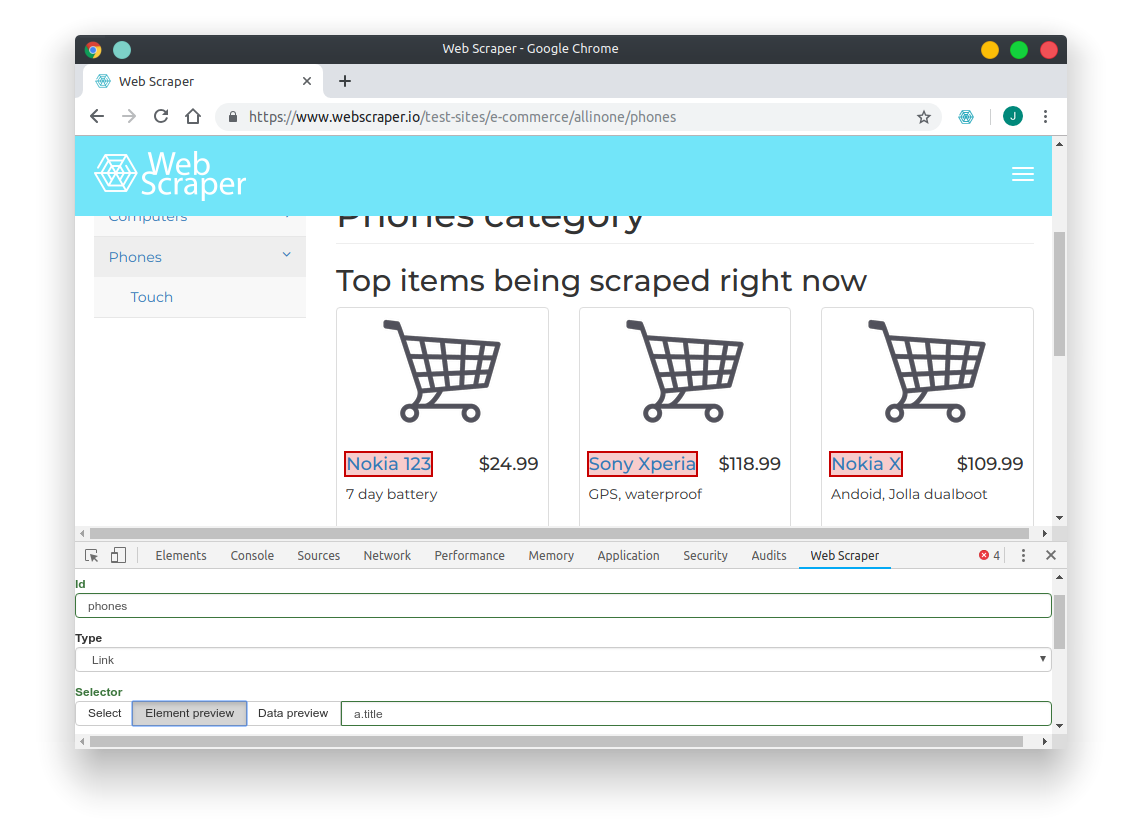
\includegraphics[width=\linewidth]{images/WebScraper.png}
	\caption[Rozšíření WebScraper]{Rozšíření WebScraper~\cite[snímek pořídil autor]{webscraper}}
	\label{fig:webScraper}
\end{figure}
\textbf{Výhody:}
\begin{itemize}
	\item jednoduchá instalace (jedná se pouze o~rozšíření do prohlížeče Google Chrome); scrapování probíhá skrze vývojářskou konzoli
	\item výběr dat pomocí klikání (inteligentní hledání vzorců/podobností na základě prvních dvou kliknutí)
	\item tutoriály jsou formou videí -- jednoduché, rychlé a naprosto postačující
	\item různé typy elementů, které vybíráme (text, odkaz, scroll down), takže lze celkem snadno projít celou doménu
	\item možnost získání dat různými formami -- přes API, jako CSV/XLS nebo do Dropboxu
	\item klávesové zkratky při výběru elementů velmi usnadňují práci
	\item možnost využít jejich cloud k~automatizaci celého procesu
	\item oproti konkurenci nabízí přehledné rozhraní a ne tak složité používání
\end{itemize}
\newpage
\textbf{Nevýhody:}
\begin{itemize}
	\item nutnost používat Google Chrome, což pro některé uživatele může být překážka
	\item nelze vyhledávat podle klíčových slov ani podle HTML nebo CSS, tudíž všechno se musí manuálně naklikat
\end{itemize}

\subsection{Dexi.io}
\begin{figure}[b]
	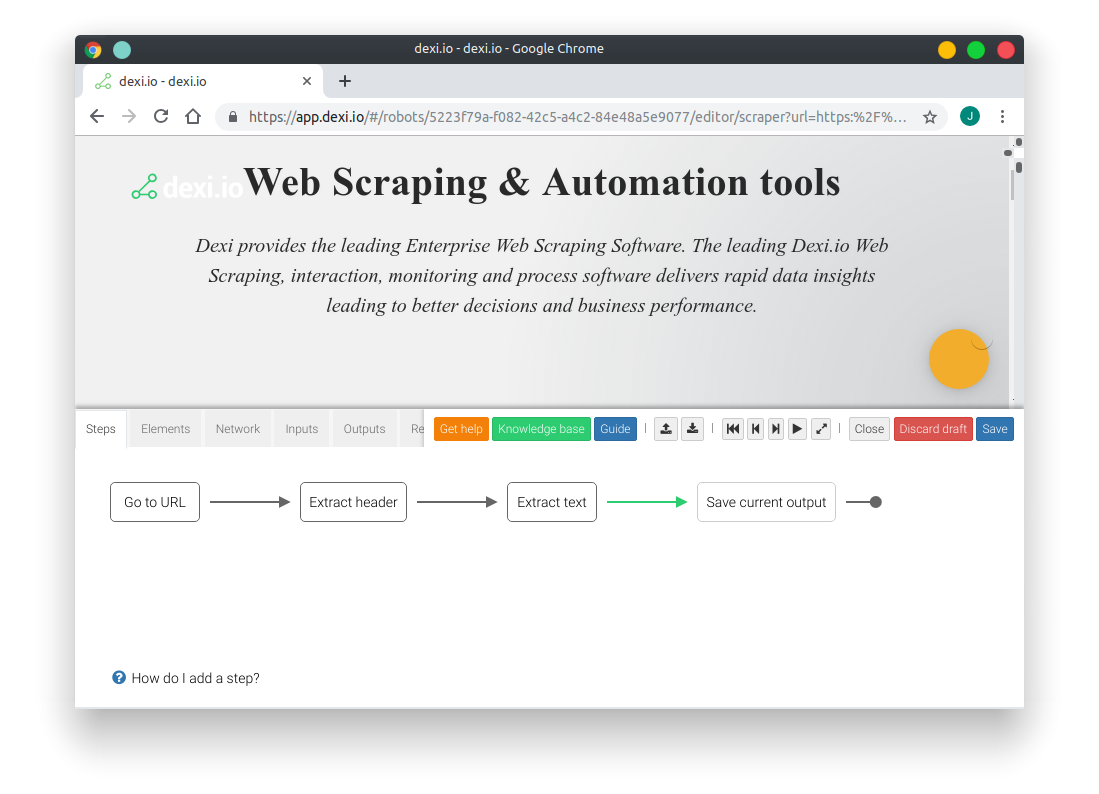
\includegraphics[width=\linewidth]{images/Dexiio.png}
	\caption[Webová aplikace Dexi.io]{Webová aplikace Dexi.io~\cite[snímek pořídil autor]{dexio}}
	\label{fig:dexi.io}
\end{figure}
\textbf{Výhody:}
\begin{itemize}
	\item bez nutnosti stahování aplikace -- vše se ovládá přes webové rozhraní
	\item výběr dat jak pomocí klikání (inteligentní hledání vzorců/podobností na základě prvních dvou kliknutí), tak pomocí HTML, CSS nebo textové shody
	\item mnoho návodů dostupných na stránkách, interaktivní rádce přímo při scrapování
	\item všechny možné druhy kliknutí, takže lze lehce projít celou doménu
	\item možnost exportovat data do CSV, JSON, XLS, získat přes API, poslat do Google Drive, Google Sheets nebo Amazon S3
	\item různé módy aplikace -- scraping, crawler, pipes (skládání menších scrape botů) a autobot (extrahování z~více stránek najednou se stejným rozlo-žením); možnost takto automatizovat celý proces.
	\item nápomocné jsou různé addony (např. na obcházení Captchy)
\end{itemize}
\textbf{Nevýhody:}
\begin{itemize}
	\item široká nabídka možností, a tak chvílí trvá, než se uživatel zorientuje
	\item placený nástroj, zadarmo je dostupná pouze týdenní zkušební verze
	\item úvodní tutoriál je velmi strohý a žádné velké seznámení s~nástrojem se nekoná
\end{itemize}

\subsection{Data Scraper}
\textbf{Výhody:}
\begin{itemize}
	\item jednoduchá instalace (jedná se pouze o~rozšíření do prohlížeče Google Chrome).
	\item velmi jednoduché ovládání a přehledné rozhraní
	\item výběr dat probíhá pomocí klikání
	\item klikáním se utváří JQuery selektor, který si uživatel může podle svého upravit a doladit tak drobné detaily, jež by jinak nutně zahltily uživatel-ské rozhraní (tedy je možné vyhledávat i~podle HTML tagů, id, CSS selektorů -- zkrátka vše, co umí klasické JQuery)
	\item různé druhy kliknutí
	\item možnost spustit na stránce libovolný JavaScriptový kód v~rámci scrapování
\end{itemize}
\textbf{Nevýhody:}
\begin{itemize}
	\item nutnost používat Google Chrome, což pro některé uživatele může být překážka
	\item oproti ostatním nástrojům se může zdát velmi chudý na různé funkce
\end{itemize}
\begin{figure}
	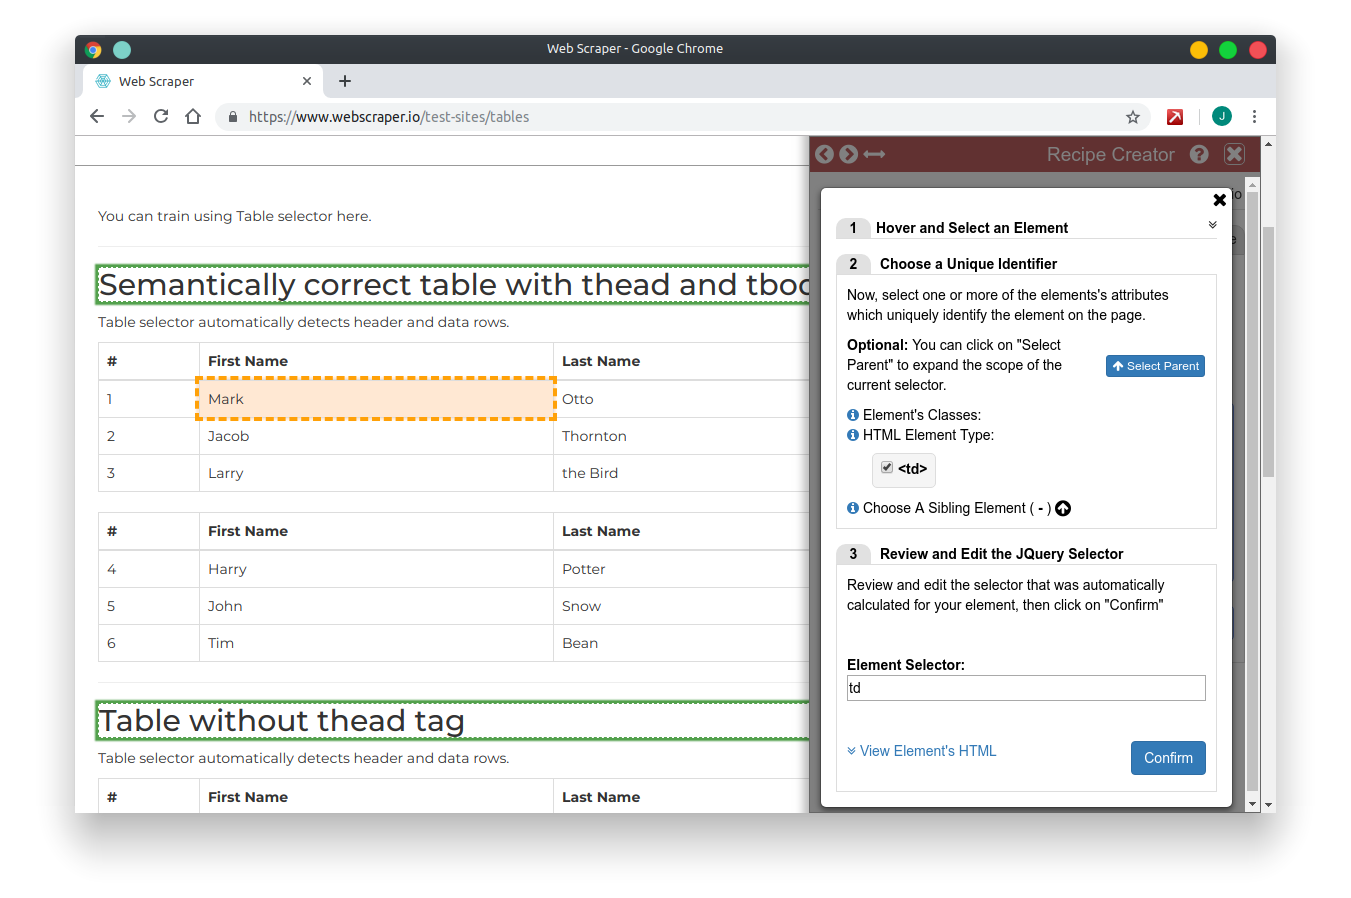
\includegraphics[width=\linewidth]{images/DataScraper.png}
	\caption[Rozšíření Data Scraper]{Rozšíření Data Scraper~\cite[snímek pořídil autor]{data_scraper}}
	\label{fig:dataScraper}
\end{figure}

% ================================================================================================

\chapter{Návrh}
V této kapitole definuji funkční i~nefunkční požadavky kladené na vyvíjený software, jež částečně vyplývají z~předchozí analýzy stávajících řešení -- problé-my konkurenčních nástrojů se snaží napravit, zároveň agregují dobré vlastnosti zmíněných aplikací. Součástí kapitoly je také diskuze případů užití výsledné aplikace. Poté se věnuji návrhu celé architektury systému a v~závěru kapitoly i~návrhu uživatelského rozhraní.

% ------------------------------------------------------------------------------------------------

\label{sec:requirements_specification}
\section{Specifikace požadavků}
Jak je patrné z~předchozí analýzy stávajících řešení, největšími neduhy, které se prolínají napříč valnou většinou aplikací, jsou \emph{těžkopádné uživatelské rozhraní}, \emph{neintuitivní ovládání} a \emph{rychlost} (nebo spíš pomalost), se kterou se uživatel dostane k~požadovaným datům. Pro aplikaci, jíž se tato práce zabývá, bude klíčové se výše zmíněným nedostatkům vyhnout a nabídnout jejich přesný opak. Také jsme se přesvědčili, že nejpříjemnější cestou je celou aplikaci ovládat přes webové rozhraní  \emph{bez nutnosti stahování a instalace}.

Na druhou stranu se lze u~konkurence i~inspirovat. Za vyzdvižení stojí určitě \emph{různé druhy výběru dat} -- \emph{klikání} přímo na stránce spolu s~inteligentním hledáním podobných prvků jistě tvoří mocný mechanismus. Avšak je potřeba zajistit i~ostatní způsoby výběru (jako je např. \emph{textová shoda, HTML tagy, CSS selektory}) pro případ, kdy je pouhé klikání zdlouhavé či nevyhovující. Rovněž široký výběr způsobů exportu dat, intuitivní klávesové zkratky a zooming in/out na prvky může uživatelům zpříjemnit práci s~nástrojem.

Neméně důležitou vlastností aplikace je také schopnost sebe sama kvalitně, ale svižně představit, \emph{seznámit uživatele s~používáním} a poskytnout mu alespoň pro začátek určité vodítko. Pro většinu ovládacích prvků by však mělo platit to stejné, co platí pro správný kód -- měly by být tzv. \emph{self-explanatory}. Tedy každému by mělo být na první pohled jasné, co který element dělá.

Pojďme si nyní všechny požadavky shrnout do několika bodů a rozdělit na funkční a nefunkční.

\subsection{Funkční požadavky}
\begin{enumerate}[F1)]
	\item Uživatelské rozhraní se skládá z~hlavní pracovní plochy, kde se bude nacházet uživatelem zadaná stránka a z~postranního panelu, obsahující všechny ovládací prvky.
	\item Postranní panel skryje tlačítka, formuláře a ostatní elementy k~ovládání aplikace do několika záložek -- tímto se na uživatele nevyvalí velké kvantum informací a možností najednou. Podle potřeby si každý rozbalí tu možnost, kterou potřebuje.
	\item Hlavní činností uživatele bude výběr elementů na jím zadané webové stránce, ze kterých bude na konci procesu vyextrahován text. Tento výběr bude probíhat následujícími způsoby:
	\begin{enumerate}[F3.1)]
		\item Kliknutím myši na požadované elementy.
		\item Na základě textové shody. Zde bude mít uživatel 4 možnosti na výběr:
		\begin{enumerate}[a)]
			\item Prvek bude vybrán, pokud jeho text začíná hledaným výrazem.
			\item Prvek bude vybrán, pokud jeho text končí hledaným výrazem.
			\item Prvek bude vybrán, pokud jeho text obsahuje hledaný výraz.
			\item Prvek bude vybrán, pokud se jeho text přesně shoduje s~hledaným výrazem.
		\end{enumerate}
		\item Pomocí CSS selektorů (tedy HTML tagy, třídy, id, hodnoty atributu, různé následnosti a vše ostatní, co CSS selektory umožňují, viz přehled CSS selektorů\footnote{\url{https://www.w3schools.com/cssref/css_selectors.asp}}).
		\item K~dispozici bude přibližování (první potomek) a oddalování (otec) momentálního výběru pomocí ikony $+$ a $-$, případně přesunutí výběru na předchozího/následujícího sourozence v~DOMu (uživatel může pomocí této funkce traverzovat napříč zanořenými prvky vše-mi směry).
		\item Na ovládacím panelu nalezneme i~tlačítka s~hotovými akcemi před-stavující šablonu pro nejpoužívanější operace (stažení všech e-mail-ových adres ze stránky, všech obrázků atd.).
	\end{enumerate}
	\item Pokud vybraným prvkem bude \textless img\textgreater~HTML tag, bude místo jeho textu extrahován atribut \textsf{src} (tedy zdroj obrázku).
	\item Po kliknutí na určitý prvek s~přidrženou klávesou \textsc{Ctrl/control} se program pokusí vybrat všechny podobné prvky na základě předchozí selekce (tzv. \emph{auto-selection}).
	\item Mezi ovládacími prvky nalezneme tlačítka \textsf{undo} a \textsf{redo}, která umožní vracet zpět provedený výběr (například v~situaci, kdy nesouhlasíme s~výběrem auto-selectu).
	\item Všechny vybrané prvky budou barevně odlišeny, aby bylo jasné, co už je připraveno k~extrakci a co ještě ne.
	\item Data z~vybraných elementů si bude možné kdykoli prohlédnout v~tzv. \textit{preview} módu -- půjde o~obyčejnou tabulku, ze které bude možné vymazat nevyhovující řádky (vymazáním řádku se odebere výběr všech relevantních prvků na stránce).
	\item Získaná data půjdou exportovat do formátů JSON, CSV, XLS.
\end{enumerate}

\subsection{Nefunkční požadavky}
\begin{enumerate}[N1)]
	\item Půjde o~webovou aplikaci běžící v~internetovém prohlížeči, tedy nebude nutná žádná instalace.
	\item Celý proces bude realizován na straně klienta -- bude se jednat pouze o~frontend, žádný backend server nebude k~dispozici.
	\item Aplikace cílí primárně na celkový zážitek uživatele -- grafické rozhraní bude přehledné a co nejjednodušší, ovládání přímočaré a intuitivní. Tento požadavek je jeden z~nejdůležitějších, neboť právě tím se nástroj odlišuje od ostatních.
	\item Důležitým aspektem je také snadná rozšiřitelnost, ať už se bude jednat o~nové možnosti výběru či přidání funkcionality web crawlingu.
	\item Čas, za který se uživatel dostane k~požadovaným datům (tedy čas, který stráví vybíráním dat; nepočítáme čas potřebný ke stažení), bude co nejmenší.
	\item Čas nutný k~samotné extrakci (od okamžiku, kdy uživatel klikne na tlačítko \textsf{Download}) nepřesáhne 5 vteřin.
\end{enumerate}

\subsection{Nice-to-have požadavky}
V~předchozích dvou sekcích jsem uvedl, jaké požadavky by aplikace v~každém případě měla splňovat a bez nichž by neměla vůbec být uvedena k~dispozici uživatelům. Pak tu jsou ale také požadavky, které rozhodně zlepšují celkovou kvalitu a pocit z~nástroje samotného, avšak nejsou již pro funkcionalitu vitální a pokud by se jejich implementace nepovedla, aplikace bude stále plno-hodnotná a připravená k~použití. Patří sem:
\begin{enumerate}[+1)]
	\item Uživatelské rozhraní aplikace nabídne intuitivní klávesové zkratky pro usnadnění práce -- \textsf{\uv{Ctrl +}} a \textsf{\uv{Ctrl -}} obstará přibližování/oddalování momentálního výběru, \textsf{\uv{Ctrl n}} a \textsf{\uv{Ctrl p}} vybere předchozího/následu-jícího sourozence vybraného prvku, apod.
	\item Postranní panel s~ovládacími prvky půjde minimalizovat (zmenšit k~při-lehlé hraně tak, aby zabíral co nejméně místa a nepřekážel v~manipulaci s~webovou stránkou) nebo přesunout na protější stranu (např. v~případě, že by zakrýval nějaké prvky na stránce).
	\item Export dat realizovatelný i~do Google Sheets, Google Drive, Dropbox.
	\item Interaktivní tutoriál, který v~rychlosti představí práci s~nástrojem.
	\item Na základě výběru dat uživatelem se vytvoří určitý filtr (textový řetězec), jenž může být ručně upraven -- půjde tak o~alternativu pro zkušenější uživatele, aniž by se zaneslo uživatelské rozhraní přehršlí možností a celé se tak znepřehlednilo.
\end{enumerate}

% ------------------------------------------------------------------------------------------------

\section{Případy užití}
\label{sec:use_cases}
Hlavní užití vyvíjeného nástroje je přímočaré -- uživatel navštíví stránku, vybere elementy nesoucí požadovaná data a exportuje je do zvoleného formátu. Mohou však nastat různé situace, kterým se věnuje následující popis.

\begin{enumerate}
	\item Uživatel chce vybrat všechny řádky tabulky nacházející se na stránce. Otevře záložku \textsf{Basics}, zapne manuální označování přepínačem s~nápisem \textsf{Selecting elements} a kliknutím myši označí první řádek tabulky. Poté s~přidrženou klávesou \textsc{Ctrl/control} klikne na druhý řádek. Tím se automaticky označí všechny řádky dané tabulky.
	\item Uživatel chce označit všechny e-mailové adresy na stránce. Otevře zá-ložku \textsf{Text search}, do pole \textsf{Contains} zadá znak \uv{@} a potvrdí stiskem klávesy \textsc{Enter}.\footnote{Často se stránky proti takovému vytěžování e-mailových adres brání například tím, že textový znak @ nahradí ikonou. V~takovém případě tento postup samozřejmě nebude fungovat.}
	\item Uživatel chce označit všechna rodná čísla, jež jsou z roku 1995. Otevře záložku \textsf{Text search}, do pole \textsf{Starts with} zadá \uv{95} a potvrdí stiskem klávesy \textsc{Enter}.
	\item Uživatel chce získat URL adresy všech obrázků z~dané stránky a ví, že se nacházejí uvnitř \textless img\textgreater~HTML tagu. Otevře záložku \textsf{CSS selectors}, zadá \uv{img} a potvrdí stiskem klávesy \textsc{Enter}.
	\item Uživatel chce vybrat nejlépe hodnocený film z~každé kategorie. Ví, že všechny filmy jsou označeny třídou \textit{movie}, přičemž první je vždy ten nejlepší z dané kategorie. Uživatel otevře záložku \textsf{CSS selectors}, zadá \uv{.movie:first-of-type} a potvrdí stiskem klávesy \textsc{Enter}.
	\item Uživatel chce vybrat určitý HTML element, ale z~nějakého důvodu to není možné (HTML struktura neumožňuje najet kurzorem na daný prvek). Vybere tak nejbližší prvek, který označit jde. Poté na něj najede kurzorem, čímž se zobrazí tlačítka pro navigaci DOMem. Pomocí nich pak může výběr přesunout na požadovaný element.
	\item Může se stát, že vybrané elementy nesplňují představy uživatele. Výběr lze vždy vrátit zpět pomocí tlačítka \textsf{undo} v~horní části ovládacího panelu. Vrácený výběr lze opět provést pomocí tlačítka \textsf{redo}. Také kliknutím myši se zapnutým ručním označováním na již vybraný element se selekce zruší.
	\item Uživatel chce vybraná data zkontrolovat před jejich stažením. Klikne na tlačítko \textsf{Preview} v~dolní části ovládacího panelu. Otevře se tabulka obsahující všechny doposud vybraná data. Nevyhovující záznamy uživatel odstraní pomocí křížku na levé straně každého řádku.
\end{enumerate}

% ------------------------------------------------------------------------------------------------

\section{Architektura systému}
Jak bylo řečeno při specifikaci nefunkčních požadavků, aplikace poběží pouze na klientské straně a veškeré procesy se vykonají v~rámci internetového prohlí-žeče (N2). Prvotní úvaha sice může vést na použití klasického \textit{frontend-backend} schématu, jenže při hlubším zamyšlení zjistíme, že to vůbec není potřeba. Z~požadavků plyne, že vybraná data budou nějakým způsobem označena (F7), tím pádem je stejně bude muset aplikace najít a zpracovat již v~prohlížeči, neboť zasílat požadavek na vzdálený server při každém kliknutí uživatele nedává smysl. Taktéž možnost kdykoli si momentálně vybraná data prohlédnout (F8) nenahrává tomuto schématu.

Celý systém se skládá z~5 hlavních komponent (viz diagram \ref{fig:conceptual_diagram}, jenž znázorňuje kompletní konceptuální model zpracovávané domény), které jsou na sobě nezávislé\footnote{Resp. pouze Controller sdružuje všechny ostatní a zajišťuje delegaci zodpovědnosti z~jedné komponenty na druhou.}:
\begin{description}
	\item [Controller,] který deleguje práci na ostatní komponenty a slouží jako pro-středník při spolupráci jednotlivých částí systému -- pokud modul A~po-třebuje nějakou akci od modulu B, zavolá příslušnou metodu v~Controlleru, i~když se často jedná pouze o~přeposlání žádosti dál. To se může jevit jako zbytečné, na druhou stranu to přináší jednu velkou výhodu. Pokud by se v~budoucnu měla potřebná metoda modulu B změnit, bylo by potřeba vykonat nějaké dodatečné akce a nebo třeba kompletně nahradit modul B nějakým jiným, stačí to udělat vždy pouze na jednom místě, a to právě v~komponentě Controller. Drží si přehled o~všech ostatních částech a má na starosti základní inicializaci.
	\item [View] představuje načtenou stránku a ovládací panel se všemi prvky uživatel-ského rozhraní. Reaguje na akce uživatele zasláním zprávy Controlleru, který rozhoduje, co se má stát dál.
	\item [Select engine] má na starosti výběr a označení požadovaných HTML elementů na stránce. Obsahuje menší komponenty:
	\begin{itemize}
		\item \emph{Selection} reprezentující výběr řádků a výběr sloupců.
		\item \emph{Selector}, jenž představuje jednotlivé způsoby výběru dat (ruční výběr, textová shoda atd.). Vybere požadované prvky na stránce a ty předá Select enginu ke zpracování.
		\item \emph{Undo-redo store}, který umožňuje zvrátit předchozí výběry nebo je naopak provést znovu.
	\end{itemize}
	\item [Data engine] zařizuje extrakci dat z~vybraných prvků na stránce (převážně tedy text, ale v~případě obrázků se jedná o~URL jejich zdroje a v~budoucnu může být snadno rozšířeno o~další možnosti) a obsahuje menší komponentu \emph{Exporter}, na kterou deleguje export dat do zvoleného for-mátu.
	\item [Preview] je komponenta reprezentující preview mód, ve kterém si uživatel může prohlédnout doposud vybraná data a ta nežádoucí z~výběru odstranit.
\end{description}
Tato modularizace je hlavním předpokladem ke splnění požadavku snadné rozšiřitelnosti (N4) a je ukázkou tzv. \emph{open-closed} principu. Podporuje nízkou provázanost a vysokou soudržnost, což je v~softwarovém inženýrství vždycky jeden z~hlavních cílů. V~případě přidání nového způsobu výběru stačí vytvořit další Selector, který prvky vybere podle požadovaných kritérií a Select engine se postará o~zpracování. Přidání automatizace bude také bez zásahu do původní implementace, neboť je jedno, jestli samotné vybírání provádí uživatel nebo jiná část programu. Pokud budeme chtít kompletně změnit uživatelské rozhraní, postačí vyměnit komponentu představující ovládací panel za novou.

Splnění nefunkčního požadavku na rychlost samotné extrakce (N6) nahrá-vá rozhodnutí vytvořit pouze frontendovou aplikaci, neboť se ušetří čas strá-vený komunikací se serverem a po načtení požadované stránky může celý scraping probíhat vlastně offline. Tím se eliminují rizika spojená s~pomalým internetovým připojením. Je ale klíčové vymyslet rychlý a efektivní způsob, jak vybraná data extrahovat v~prohlížeči -- tento úkol je ponechán na konkrétních implementacích.

\begin{figure}
	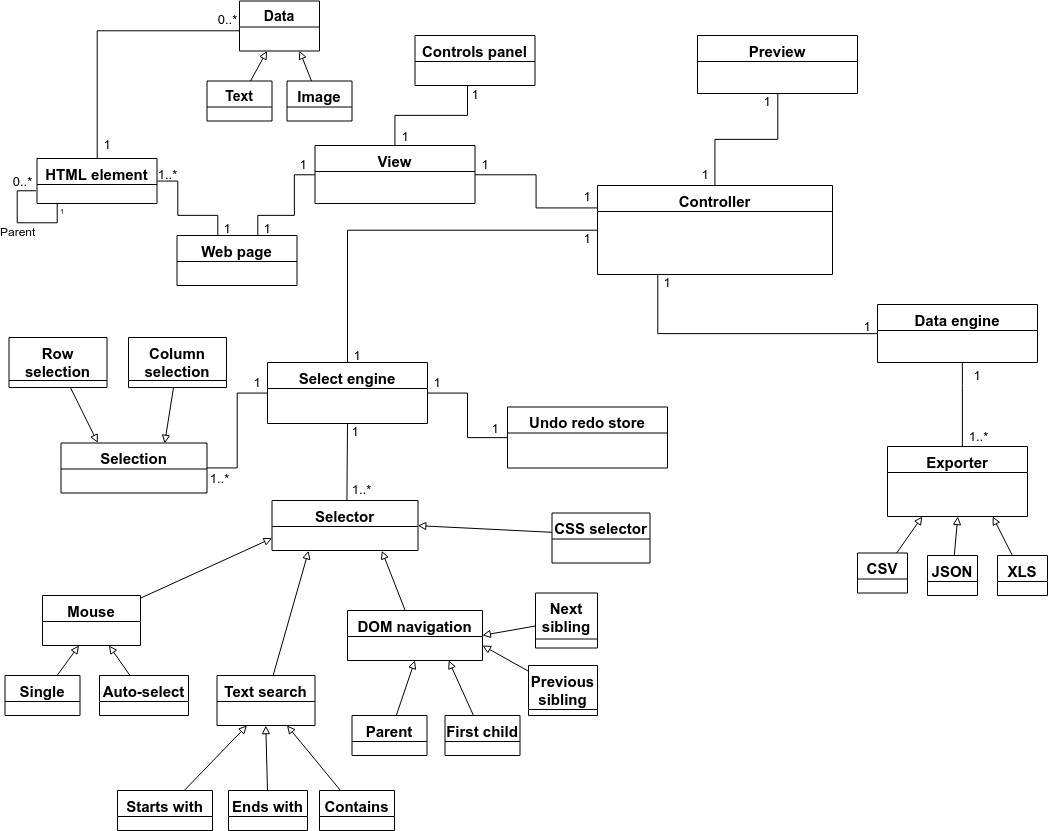
\includegraphics[width=\linewidth]{images/conceptual_diagram.png}
	\caption[Analytický doménový model]{Diagram představující analytický doménový model}
	\label{fig:conceptual_diagram}
\end{figure}

% ------------------------------------------------------------------------------------------------
\newpage
\section{Návrh uživatelského rozhraní}
Při návrhu uživatelského rozhraní je nutné zohlednit ten nejdůležitější aspekt vyvíjené aplikace, a sice intuitivní, jednoduché a přehledné ovládání (N3), kterým se tento nástroj chce odlišit od stávajícího softwaru zabývající se stejnou problematikou. V~potaz je nutné brát i~požadavek na co nejmenší čas strávený vybíráním dat (N5) -- od uživatele je potřeba co nejmenší počet kroků.

Dle požadavku F1 je aplikace rozdělena na pracovní plochu s~uživatelem zadanou stránkou a postranní panel, skrz který probíhá veškeré ovládání. Dle F2 je pak panel rozdělen na záložky obsahující jednotlivé způsoby výběru. V~horní části panelu nalezneme ovládací tlačítka akcí undo a redo. Zbývá už jen tlačítko \textsf{Preview} a \textsf{Download} spolu s~výběrem formátu exportu.

Následující obrázky \ref{fig:scraper_main_wireframe} a \ref{fig:scraper_text_search_wireframe} představují wireframy uživatelského rozhraní aplikace.
\begin{figure}[h]
	
\includegraphics[width=\linewidth]{images/main_wireframe.png}
	\caption{Návrh ovládacího panelu aplikace}
	\label{fig:scraper_main_wireframe}
\end{figure}
\begin{figure}
	
\includegraphics[width=\linewidth]{images/text_search_wireframe.png}
	\caption{Návrh textového výběru}
	\label{fig:scraper_text_search_wireframe}
\end{figure}

% ================================================================================================


\chapter{Realizace}
Tato část se zabývá naplněním funkčních a nefunkčních požadavků z~minulé kapitoly z~hlediska konkrétní implementace. Diskutuji problémy a zádrhely, které nastaly při vývoji aplikace (především pak podrobně vysvětluji, proč bylo upřednostněno rozšíření do prohlížeče před webovou aplikací), stejně tak jejich možná řešení a proč bylo zvoleno zrovna dané rozhodnutí. Dále představuji výslednou aplikaci, popisuji způsob jejího používání a v~poslední sekci nalezneme realizaci jednotlivých komponent systému.

% ------------------------------------------------------------------------------------------------

\label{sec:possible_solutions}
\section{Diskuze možných řešení}
Původní záměr byl vytvořit webovou aplikaci, neboť věřím, že nikdo v~dnešní době nechce cokoli stahovat a instalovat. Vzhledem k~důrazu vyvíjeného ná-stroje kladeného na jednoduchost a rychlost používání je tak webová aplikace jasnou volbou, jelikož se jedná o~nejpřímočařejší řešení a pro uživatele určitě nejpohodlnější.

Návrh tedy předpokládal jednoduchou webovou aplikaci s~hlavní obrazovkou, kde by byla zobrazená uživatelem zadaná stránka a postranním panelem, který by obsahoval veškeré ovládací prvky. Jasným řešením tak byl HTML iframe, který reprezentuje vnořený kontext procházení (kontext procházení si můžeme představit jako jedno okno/záložku prohlížeče) -- tedy umožňuje zobrazit HTML dokument uvnitř jiného HTML dokumentu~\cite{iframe}.

Ač se toto zprvu zdálo jako ideální řešení, hned v~úvodu jsem narazil na stěžejní implementační problém -- z~bezpečnostních důvodů existuje HTTP hlavička \emph{X-Frame-Options}, která určuje, kdo může danou stránku vložit do iframe tagu a zobrazit ji v~rámci své vlastní stránky~\cite{x_frame_options}. Spousta webových stránek nastavuje tuto hlavičku tak, aby nebylo možné jejich stránky vkládat do iframů, čímž se brání tzv. \emph{clickjacking} útokům~\cite{clickjacking}~\cite{clickjacking_defense}. Jenže to představuje v~podstatě neřešitelný problém, neboť HTTP hlavičky se v~prohlížeči nedají nijak obejít a dá se předpokládat, že toto blokování bude provádět mnoho stránek.

Možnou alternativou by bylo stáhnout veškerý obsah ze zadané domény (HTML, CSS, JavaScript, všechny assety jako obrázky apod.), ten sestavit dohromady a poskytovat z~vlastního serveru pouze danému uživateli. V~podstatě by tak došlo k~vyscrapování všech dat z~cílové domény a uživatel by již pouze odfiltroval informace, o~které nemá zájem. To je ale nevhodné hned z~několika důvodů -- jednak by byla uživatelům prezentována stránka, která ve skutečnosti není tou, za kterou se vydává; mohlo by docházet k~porušení copyrightu a autorských práv a v~neposlední řadě by složitost takového řešení naprosto neodpovídala poměrně přímočarému úkolu výsledné aplikace.

Na problém se však lze dívat i~opačně a základní myšlenku invertovat, což nás dovede k~použitému řešení. Pokud není možné vložit stránku do webové aplikace, je nutné vložit aplikaci do požadované stránky. To lze elegantně vyřešit pomocí rozšíření do internetového prohlížeče Google Chrome -- tzv. \emph{Chrome-extension}.

% ------------------------------------------------------------------------------------------------

\section{Použité technologie}	
\label{sec:used_technology}
Celé řešení zadaného problému je tedy nakonec implementováno jako rozšíření do internetového prohlížeče Google Chrome (jehož popisu se věnuji níže). Z~tohoto důvodu je zvoleným programovacím jazykem čistý JavaScript, resp. ECMA-Script 2018 verze 9. Dále je použit značkovací jazyk HTML k~definici struktury celého ovládacího panelu a zbylých kontrolních prvků spolu s~CSS jazykem určujícím styl zobrazení jednotlivých elementů. K~testování aplikace byl použit JavaScriptový testovací framework Jest. Jako verzovací sytém jsem použil Git.

\subsection{Rozšíření do prohlížeče Google Chrome}
Chrome-extensions se skládají z~několika různých komponent (viz oficiální dokumentace\footnote{\url{https://developer.chrome.com/extensions}}). Nás budou zajímat následující tři:
\paragraph{Background script} je základní komponenta (můžeme si ji představit jako takový backend celého rozšíření), která se vykoná při každém spuštění prohlí-žeče. Zde je možné registrovat obsluhy různých událostí (např. když se otevře nová záložka v~prohlížeči nebo když je dané rozšíření poprvé nainstalováno). 
\paragraph{Browser action} představuje tlačítko rozšíření umístěné v~hlavním panelu nástrojů prohlížeče Google Chrome (vedle pole pro zadávání adresy). Po kliknutí na něj je vypuštěna událost mířící do background scriptu, kde se odehrává následné zpracování.
\paragraph{Content script}\label{def:content_script} je zajisté tím nejsilnějším mechanismem, které Chrome extensions nabízí. Zároveň je nejdůležitější částí tohoto ekosystému, jenž nás bude zajímat. Jedná se o~kód, který je vložen do požadované stránky a spustí se v~rámci jejího kontextu. To znamená, že každý takto vložený skript má \emph{kompletní přístup k~DOMu} dané stránky i~všem ostatním skriptům. Stane se validní součástí stránky, může \emph{vytvářet, mazat nebo měnit prvky}, a sice do doby, než je stránka obnovena a znovu načtena.

% ------------------------------------------------------------------------------------------------

\section{Představení nástroje}
Před používáním nástroje je nutné si uvědomit jednu velmi podstatnou věc -- co je výsledek, který očekáváme na konci. Jak mají vypadat data, která plánujeme extrahovat, jakou mají mít podobu? V~rámci našeho nástroje se bude ve výsledku jednat vždy o~\emph{tabulku}. Toto je nezbytné pro pochopení celého procesu.

Nyní se můžeme podívat na použití aplikace (předpokládejme, že rozšíření je již nainstalované v~prohlížeči):
\begin{enumerate}
	\item Uživatel navštíví stránku, ze které si přeje extrahovat dat.
	\item Klikne na ikonu rozšíření nacházející se v~pravém horním rohu prohlížeče, v~hlavním panelu nástrojů.
	\item Zobrazí se hlavní ovládací panel a aplikace je připravena k~výběru dat, viz obrázek \ref{fig:scraper_control_panel}.
\end{enumerate}
\begin{figure}
	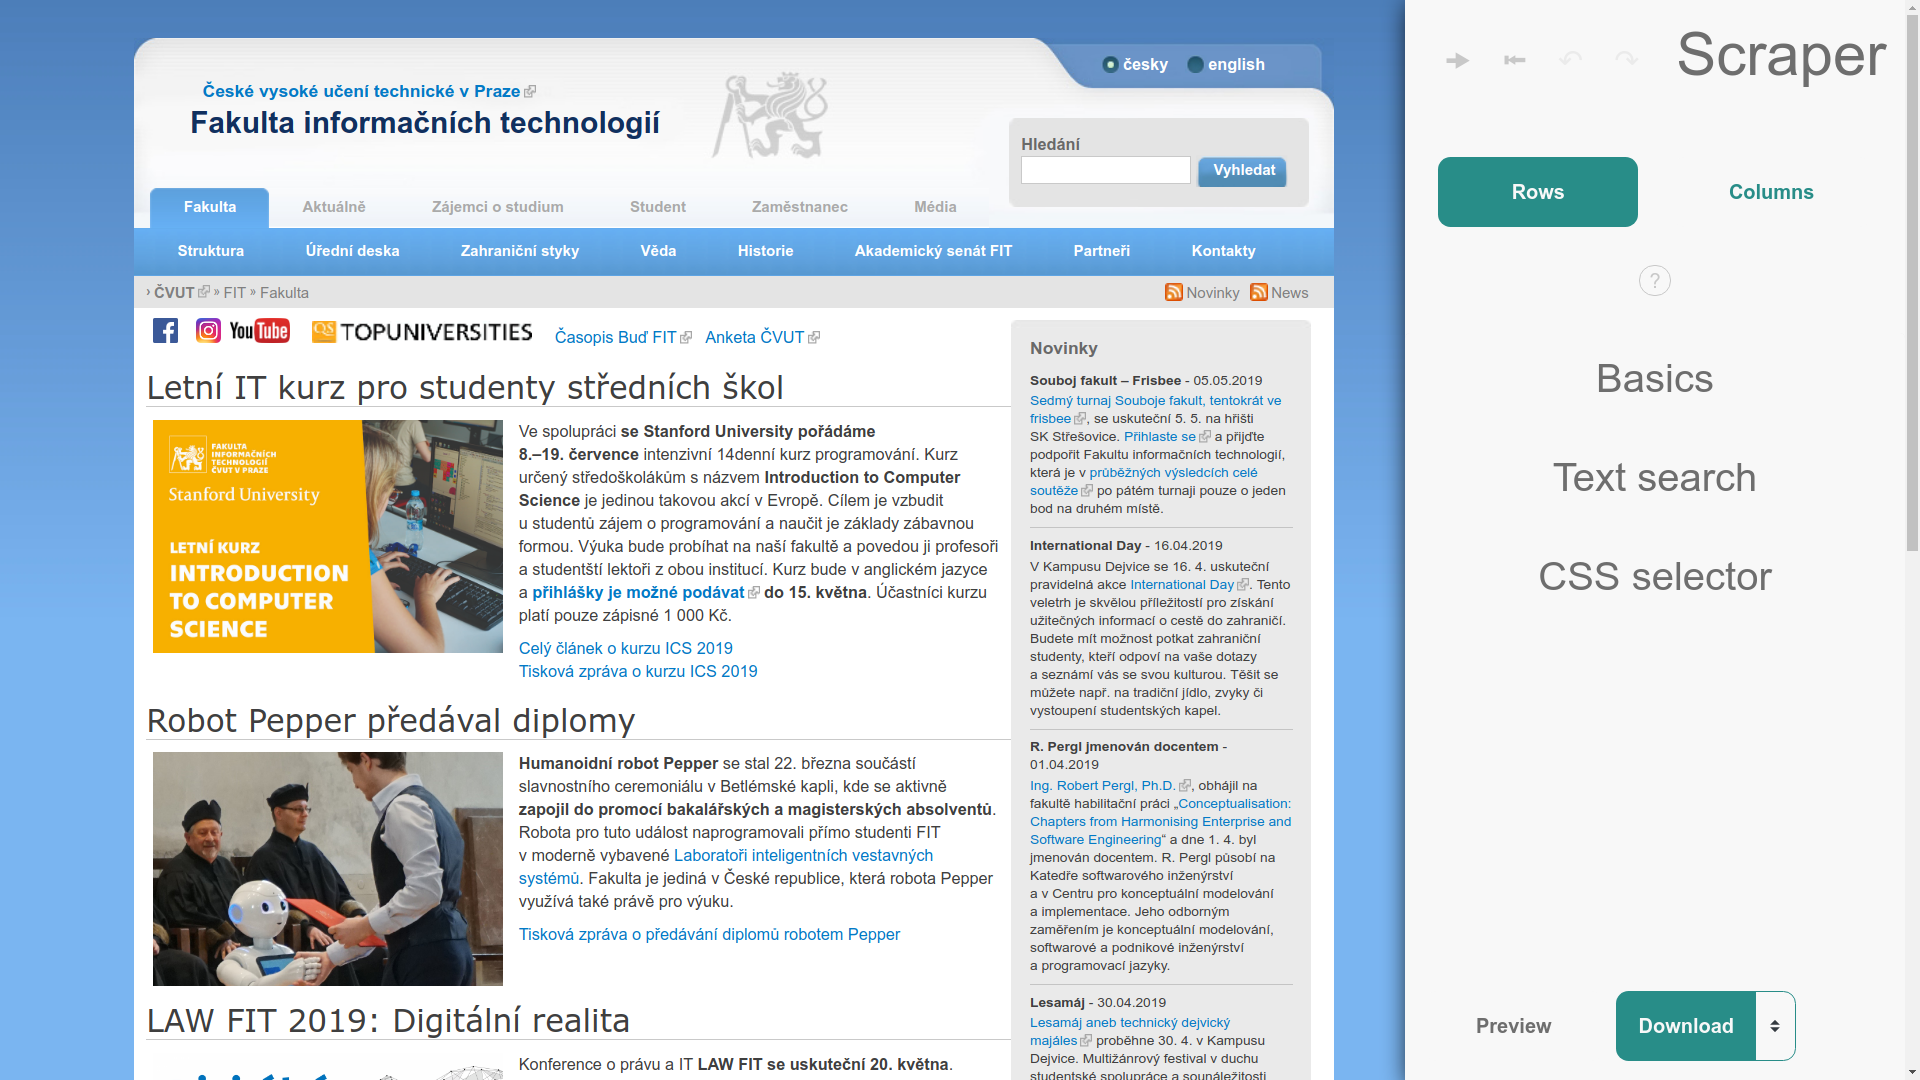
\includegraphics[width=\linewidth]{images/Scraper_control_panel.png}
	\caption{Ovládací panel aplikace}
	\label{fig:scraper_control_panel}
\end{figure}

Jak již bylo zmíněno v~úvodu, výsledná data budou ve formě tabulky, tedy musíme vybrat, které elementy na stránce budou reprezentovat řádky výsledné tabulky a které budou reprezentovat sloupce, viz obrázek \ref{fig:scraper_rows_cols}. K~tomu slouží dvě velká tlačítka \textsf{Rows} a \textsf{Columns}, kterými se přepíná výběr právě mezi řádky a sloupci. Doporučený postup je nejdřív vybrat řádky\footnote{To budou nejčastěji různé \uv{kontejnery}, které sdružují data jedné entity dohromady -- jako příklad lze uvést kartu produktu v~přehledu produktů e-shopu.} a poté uvnitř těchto větších elementů vybírat sloupce\footnote{To může být například cena nebo jméno daného produktu.}.
\begin{figure}
	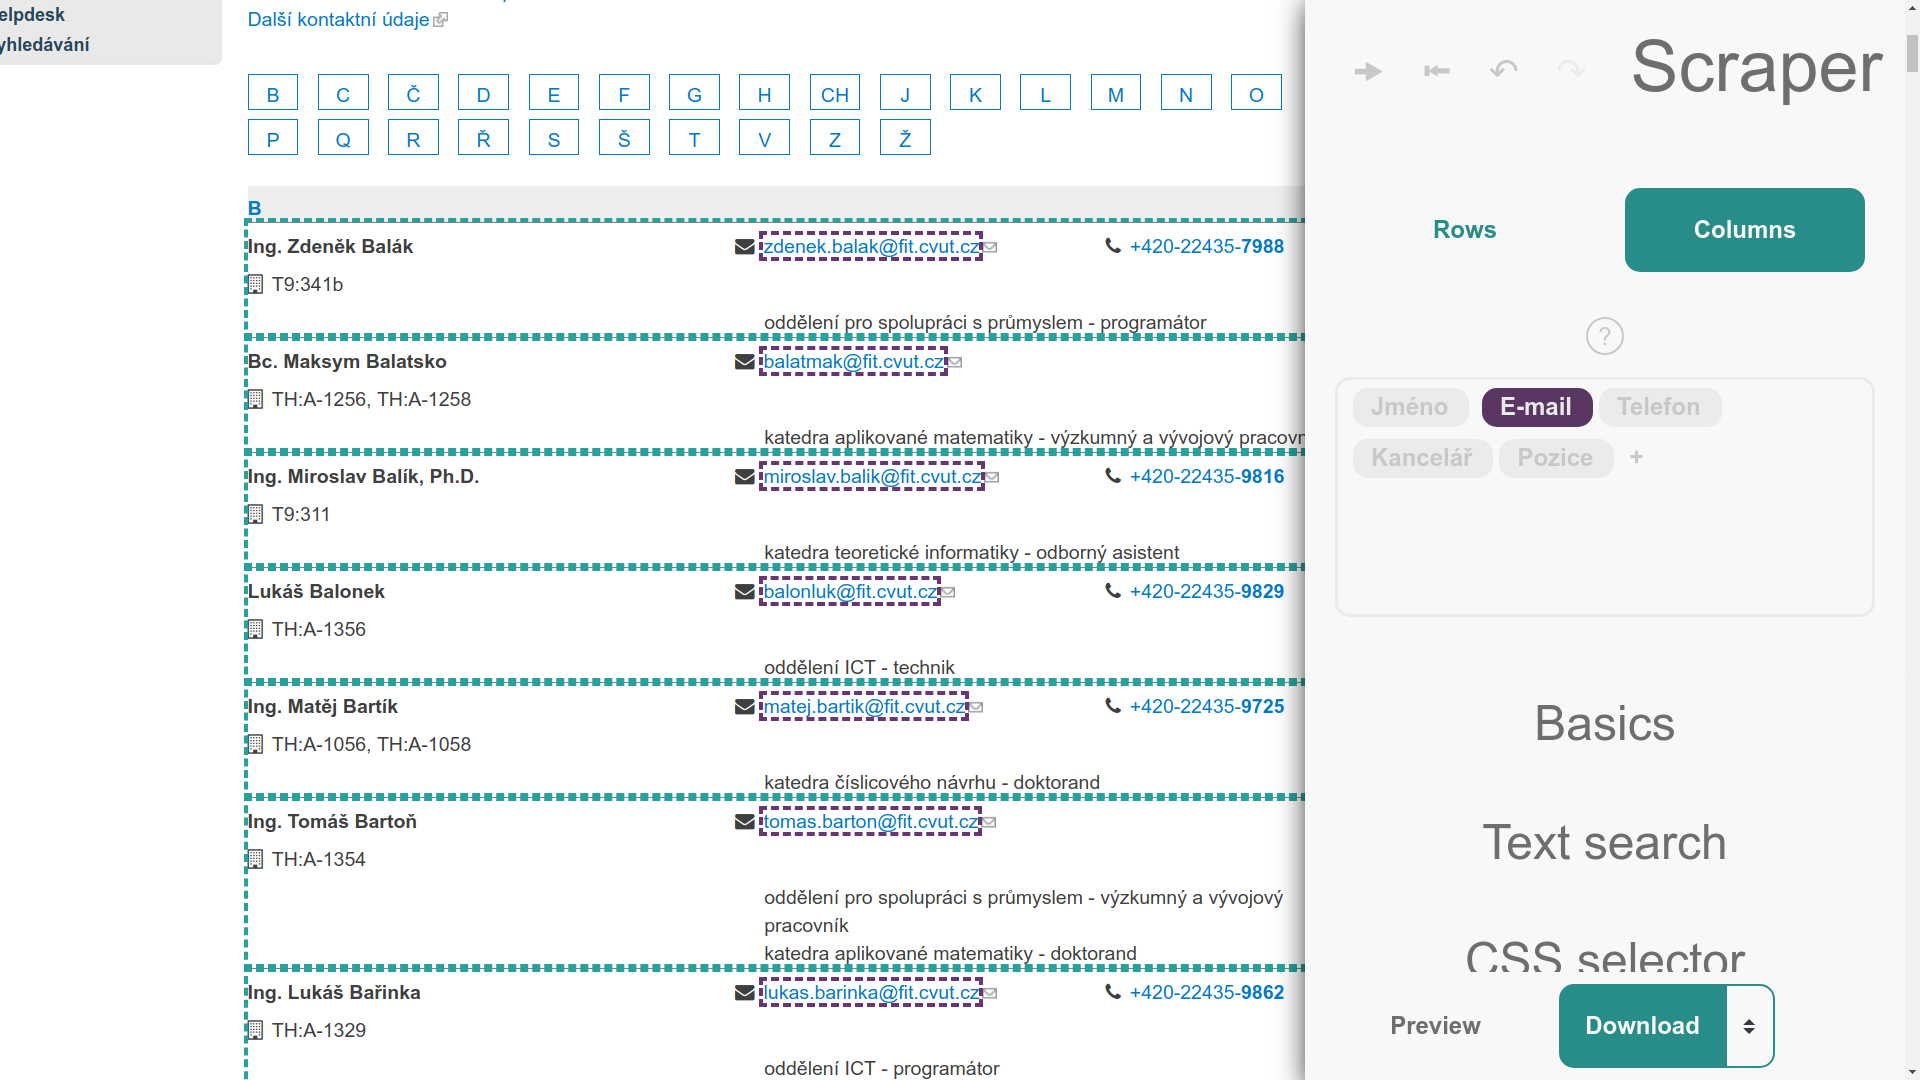
\includegraphics[width=\linewidth]{images/Scraper_rows_cols.png}
	\caption[Výběr řádků a sloupců]{Výběr řádků (tyrkysově) a sloupců (vínově)}
	\label{fig:scraper_rows_cols}
\end{figure}

Dle zadání v~kapitole \hyperref[sec:requirements_specification]{Návrh, sekce Specifikace požadavků}, probíhá selekce třemi způsoby -- ruční označování prvků, hledání na základě textové shody a výběr pomocí CSS selektorů. Tyto tři druhy výběru jsou stejné jak pro výběr řádků, tak pro výběr sloupců. Jakýkoli výběr lze vzít zpět nebo následně provést znovu pomocí tlačítek \textsf{Undo} a \textsf{Redo} v~horní části nástroje. Následuje popis každého ze způsobů výběru:
\begin{description}
	\item[Ruční označování] probíhá klikáním myši na požadované elementy a zapíná se přepínačem nacházejícím se na kartě \textsf{Basics}. Pokud uživatel při vybí-rání podrží klávesu \textsc{Ctrl}, aplikace se pokusí vybrat všechny podobné prvky na základě předchozího kliknutí. Kliknutím na již označený element se výběr zruší.
	
	Největší část výběrů bude představovat právě tento způsob.
	
	\item [Textová shoda] se nalézá na kartě \textsf{Text search}, která se skládá ze tří samostatných formulářů. Uživatel má možnost vybrat všechny elementy na stránce, jejichž text buď:
	\begin{enumerate}[a)]
		\item začíná daným výrazem,
		\item končí daným výrazem,
		\item obsahuje daný výraz nebo se mu přímo rovná.
	\end{enumerate}
	Tento způsob se osvědčí například v~případě, kdy chceme vybrat všechny e-mailové adresy na stránce -- stačí hledat prvky, které obsahují zavináč.
	\item [CSS selektory] najdeme na kartě s~názvem \textsf{CSS selectors} a jedná se o~jednoduché textové pole, které přijímá libovolný CSS selektor. Můžeme tedy pomocí něj vybírat na základě HTML tagů (\textsf{jmenoTagu}), tříd (\textsf{.jmenoTridy}), atributů (\textsf{[atribut=hodnota]}), různé následnosti (\textsf{otec $>$ syn $+$ naslednik}) a zkrátka vše, co CSS selektory umí, viz přehled selektorů \footnote{\url{https://www.w3schools.com/cssref/css_selectors.asp}}.
	
	Toto je jistě nejsilnější z~uvedených způsobů, jelikož s~ním jde vybrat libovolná skupina prvků, avšak předpokládá alespoň základní znalost HTML, CSS a především struktury stránky. Je tedy spíš pro pokročilejší uživatele.
\end{description}

\begin{figure}
	\centering
	\begin{minipage}{.5\linewidth}
		\centering
		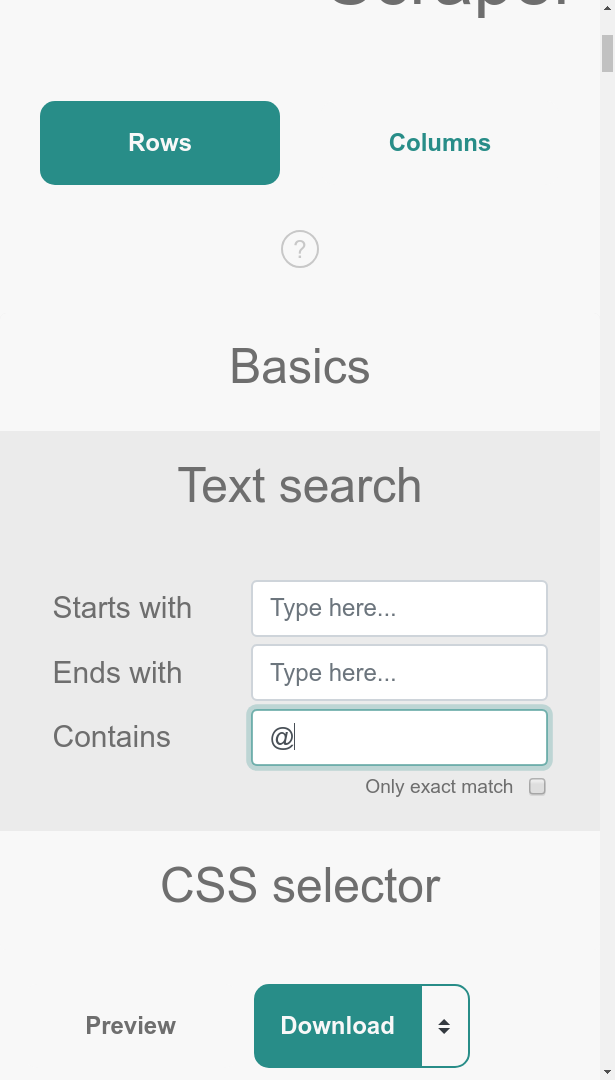
\includegraphics[width=.75\linewidth]{images/Scraper_text_search.png}
		\caption[Výběr na základě textové shody]{Výběr na základě \newline textové shody}
		\label{fig:scraper_text_search}
	\end{minipage}%
	\begin{minipage}{.5\linewidth}
		\centering
		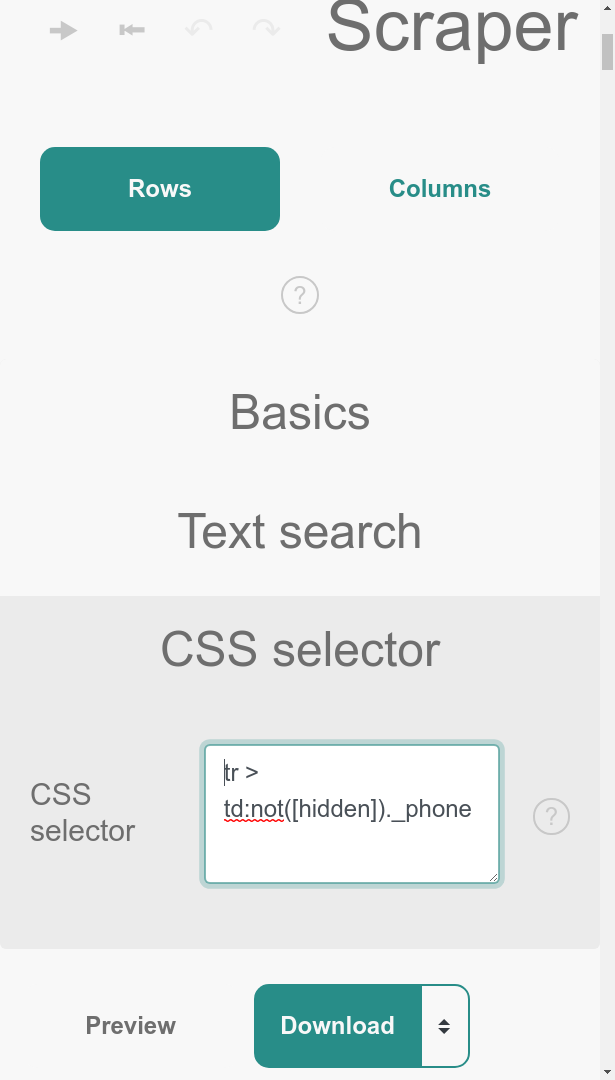
\includegraphics[width=.75\linewidth]{images/Scraper_css_selector.png}
		\caption[Výběr s~pomocí CSS selektoru]{Výběr s~pomocí CSS \newline selektoru}
		\label{fig:scraper_css_selector}
	\end{minipage}
\end{figure}

\newpage
Může se stát, že požadovaný element nejde označit ručně. Pro tyto případy je každý vybraný prvek opatřen čtveřicí tlačítek, která se objeví, pokud uživa-tel najede kurzorem na daný element, viz obrázek \ref{fig:scraper_dom_navigation}. Tlačítko \textsf{$+$} posune označení na prvního syna prvku, \textsf{$-$} na otce, \textsf{$\leftarrow$} na předchozího sourozence a tlačítko \textsf{$\rightarrow$} na následujícího sourozence. Tímto způsobem může uživatel traverzovat napříč celým DOMem a vybrat tak libovolný prvek.

Někdy je také vhodné mít ovládací panel na levé straně, případně ho minimalizovat, aby nezabíral místo a nepřekrýval prvky, které by mohl uživatel chtít vybrat. K tomu slouží dvě šipky v horní části nástroje vedle ikon pro akce undo a redo.
\begin{figure}
	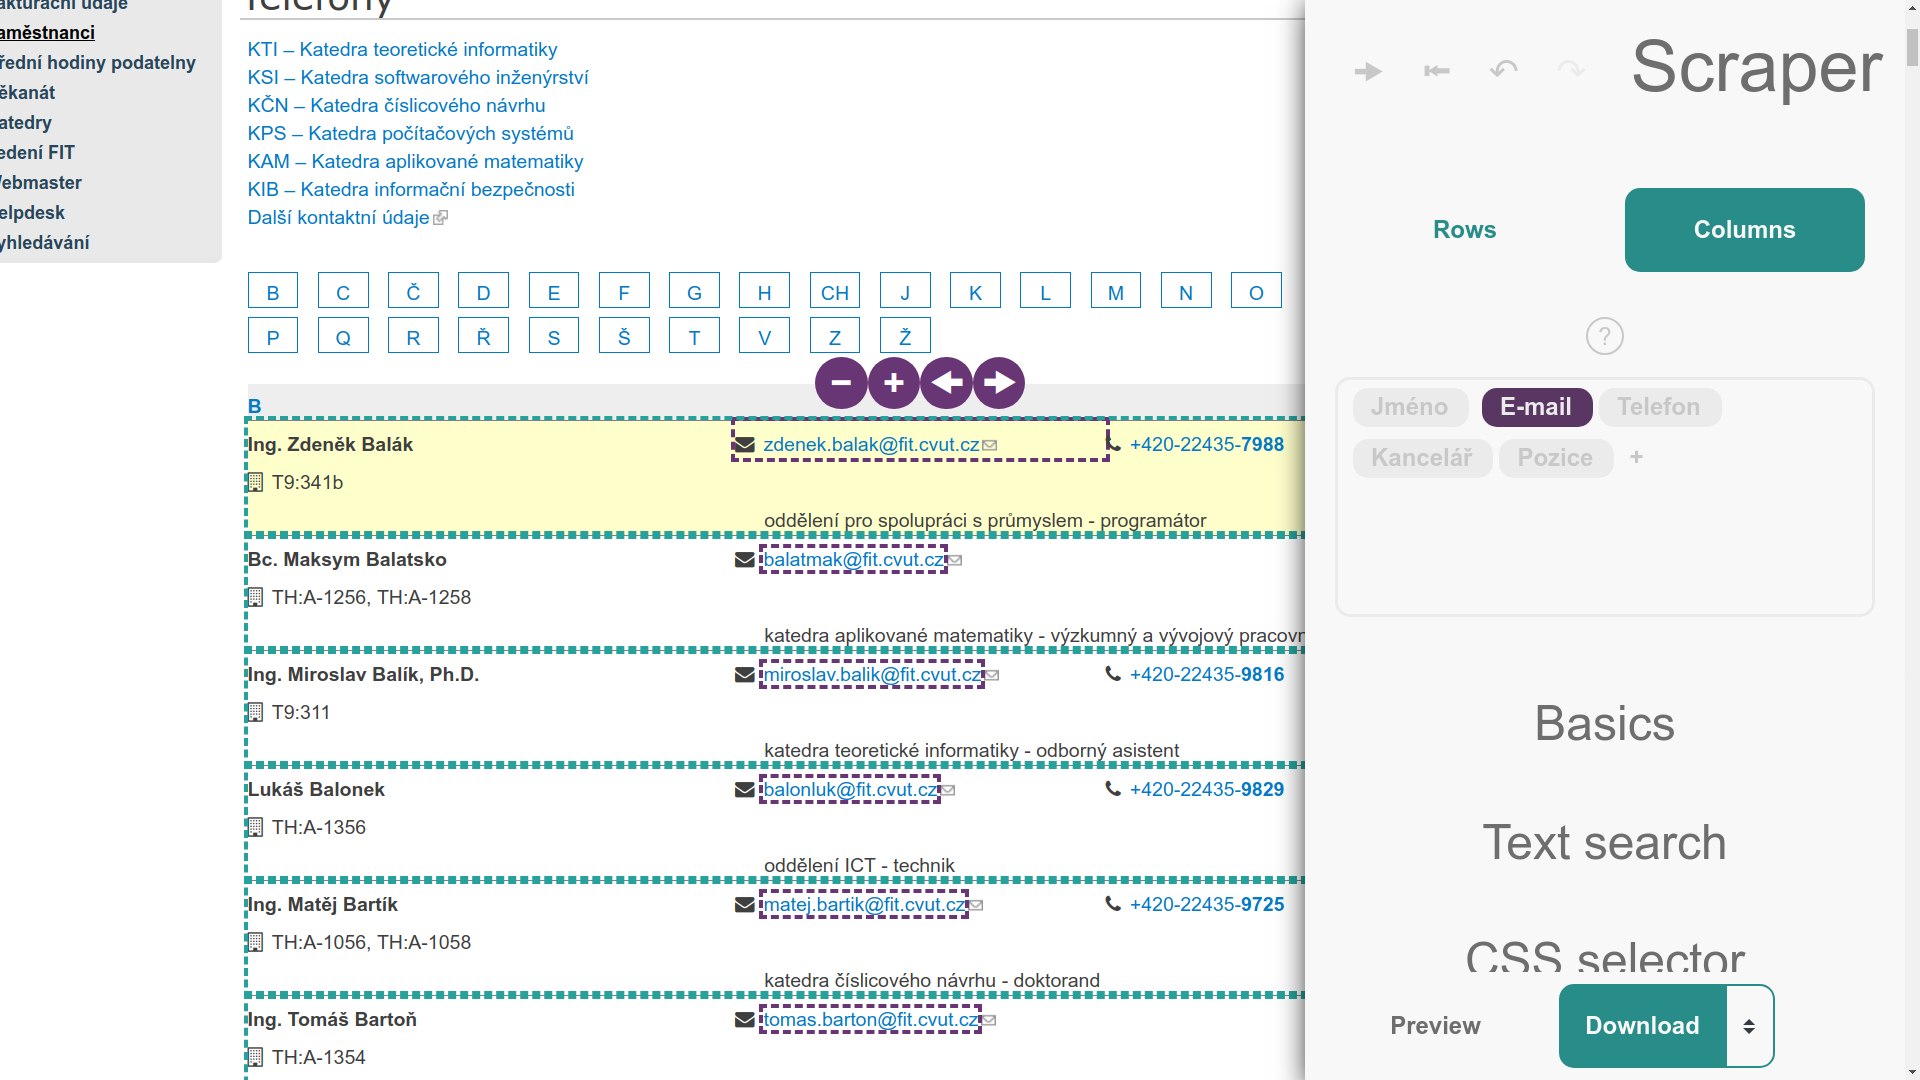
\includegraphics[width=\linewidth]{images/Scraper_dom_navigation.png}
	\caption{Ovládací prvky navigace výběru}
	\label{fig:scraper_dom_navigation}
\end{figure}

Poté, co jsme s~výběrem hotovi, je možné data prohlídnout v~tzv. \textit{Preview módu}. Zobrazí se tabulka obsahující námi zadané řádky a sloupce\footnote{Nutno podotknout, že prvky označené jako sloupce, které se \emph{nenacházejí} uvnitř prvku označeného jako řádek, nebudou zahrnuty do výsledku.}. V~tuto chvíli je možné zkontrolovat veškerá extrahovaná data a případně vyřadit ta, která nevyhovují našim potřebám pomocí křížku na levé straně každého řádku (ten se objeví až po najetí kurzorem na daný řádek), viz obrázek \ref{fig:scraper_preview_mode}. Vyřazení záznamu způsobí zrušení výběru elementů, které obsahují příslušná data.
\begin{figure}
	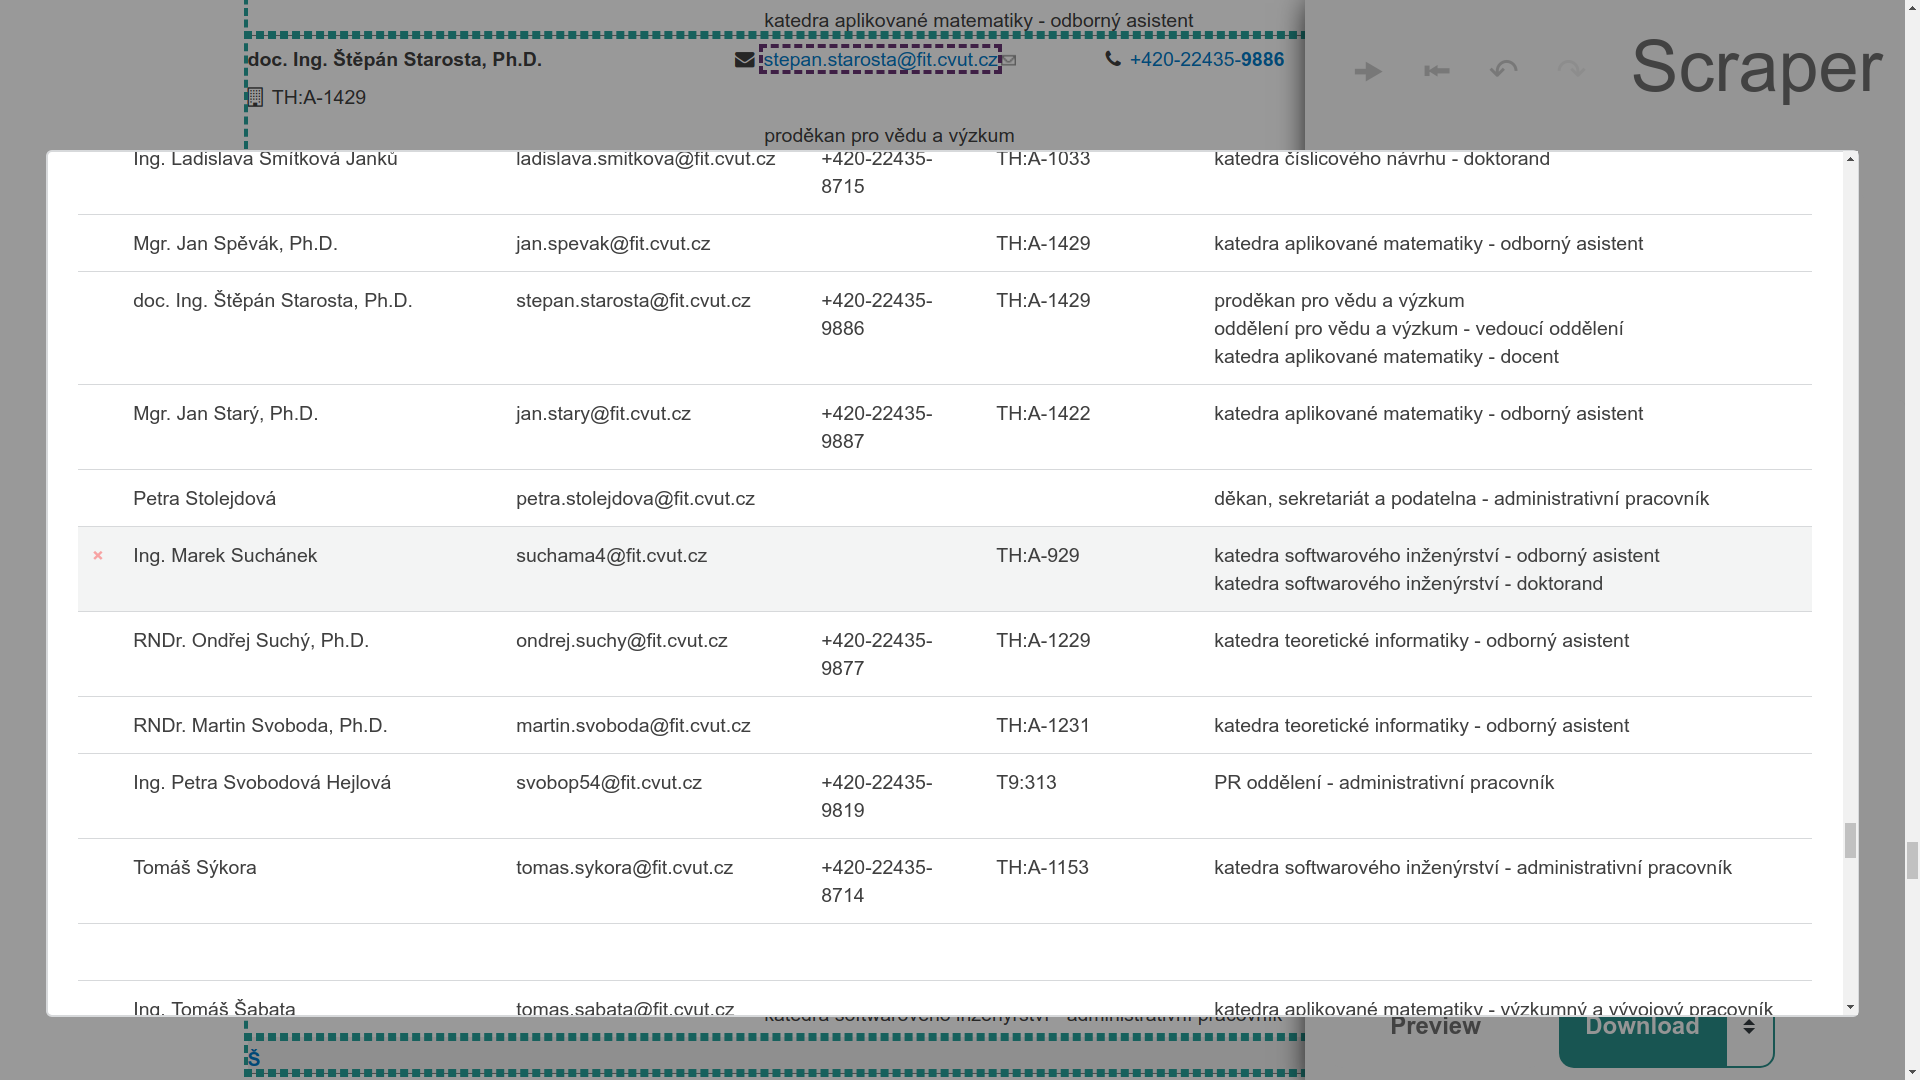
\includegraphics[width=\linewidth]{images/Scraper_preview_mode.png}
	\caption{Tabulka obsahující náhled extrahovaných dat}
	\label{fig:scraper_preview_mode}
\end{figure}

Na závěr stačí pomocí rozbalovacího výběru zvolit formát, do kterého chceme data exportovat (na výběr je CSV a JSON) a kliknout na tlačítko \textsf{Download}.

% ------------------------------------------------------------------------------------------------

\section{Implementace zvoleného řešení}

\subsection{Inicializace a spuštění}
Jak již bylo řečeno v~úvodu této kapitoly, použité řešení spočívá ve vložení ovládacího panelu do libovolné stránky. To umožňuje právě komponenta \hyperref[def:content_script]{content script}, jež byla zmíněna v sekci \ref{sec:used_technology} Použité technologie. Tuto komponentu reprezentují v aplikaci komponenty Controller, SelectEngine a DataEngine. Spuštění aplikace vypadá následovně:
\begin{enumerate}
	\item Po instalaci rozšíření (a každém jeho spuštění) do prohlížeče Google Chrome je vykonán kód, který je obsažen v~background scriptu. Zde se nachází obsluha vyzývající content script k~zobrazení nebo schování ovládacího panelu.
	\item Když je rozšíření aktivní, do \emph{každé} načtené stránky je vložen content script, jenž poslouchá zprávy od background scriptu.
	\item Kliknutím na ikonu rozšíření v~hlavním panelu nástrojů je vyvolána událost, na kterou reaguje background script -- aktivnímu oknu/záložce zašle zprávu, aby byl otevřen ovládací panel. 
	\item Tu odchytí content script, jenž na dané stránce poslouchá a vloží do těla stránky nový iframe, do něhož načte HTML dokument, který představuje samotný ovládací panel. Při dalších žádostech je iframe pouze skryt/zob-razen.
	\item Vhodným nastavením příslušných CSS vlastností je iframe umístěn na boční straně prohlížené stránky a nabývá formy ovládacího panelu. 
\end{enumerate}
Obrázek \ref{fig:scraper_control_panel} ilustruje, jak ovládací panel vypadá po vložení do stránky.

\subsection{Výběr dat}
\label{sec:data_selection}
Výběr dat má na starosti třída SelectEngine, která téměř všechnu svou práci deleguje na třídy Selection a Selector. 

\begin{description}
	\item[Selection] definuje, jakým způsobem probíhá samotný výběr řádků/sloup-ců -- od Select enginu dostane pole HTML elementů a \emph{každému přidá patřičnou CSS třídu}\footnote{Řádky mají jinou třídu než sloupce, navíc každý řádek/sloupec má své vlastní pořadové číslo, jež je obsažené v této třídě, např. \textsf{scraping-col-1}.}. Ta zajistí, že jsou všechny vybrané elementy na stránce barevně ohraničeny a je tak jasné, které prvky jsou již označeny. Přidávat a odebírat CSS třídy nám umožňuje fakt, že třída SelectEngine (a potažmo její podtřída Selection) představuje výše zmíněný \emph{content script}, díky čemuž máme kompletní přístup k DOMu navštívené stránky.
	
	Každý prvek, předtím než je vybrán, je zároveň zkontrolován, zdali je pro výběr vhodný (to znázorňuje fragment \textsf{opt} v diagramu \ref{fig:sequence_diagram}) -- především, jestli je viditelný. Ověřuje se tedy existence HTML atributu \textsf{hidden}, kladnost atributů \textsf{offsetWidth, offsetHeight} a CSS vlastnosti \textsf{display} a \textsf{opacity}. Nemělo by se tak stát, že aplikace vybere něco, co uživatel nemůže vidět.
	
	\item[Selector] najde požadované prvky na stránce a předá je rodičovské třídě SelectEngine k označení, viz diagram \ref{fig:sequence_diagram}. Jednotlivé Selectory fungují následovně:
	\begin{itemize}
		\item MouseSelector -- po zapnutí jsou na celém dokumentu zaregistro-vány dva handlery. První reaguje na události \emph{mouseover}/\emph{mouseout} a zajišťuje, že je daný HTML element barevně podbarven, pokud na něj uživatel najede kurzorem myši. Druhý pak naslouchá události \emph{click}. Pokud nastane, přeruší její probublávání do dalších handlerů a zabrání provedení defaultní akce. Tím je zajištěno, že kliknutí myší se zapnutým MouseSelectorem pouze označí vybraný prvek, ale nespustí žádnou akci, kterou by normálně spustit mělo.\footnote{Jako příklad si můžeme představit kliknutí na odkaz, které defaultně přesměruje uživatel na adresu obsaženou v atributu \textsf{href}.}
		
		Selekce všech podobných prvků na základě momentálního a před-chozího výběru (auto-select) není nic jiného než hledání společných vlastností těchto dvou elementů -- porovnává se jméno HTML tagu, třídy, které element nese a všechny jeho atributy. Vlastnosti, v nichž se elementy shodují, vytvoří CSS selektor, podle kterého jsou vybrány všechny podobné prvky.
		\item TextSelector -- obdrží hledaný řetězec a poté iteruje přes všechny HTML elementy na stránce od toho nejvyššího (\textless \textsf{body}\textgreater) po ty nejvíce zanořené. Pokud narazí na prvek, jenž neobsahuje žádný text, pokračuje ve zpracování následujícího elementu. Pokud má prvek nějaké potomky, zařadí ho do fronty procházení, jinak porovná jeho text s hledaným řetězcem a v případě shody ho uloží do pole prvků určených k označení. Hledání shody nerozlišuje velká a malá písmena.
		\item CSSSelector -- obdrží libovolný CSS selektor a pomocí volání metody \verb|document.querySelectorAll()| vybere všechny odpovídající prvky, které předá k označení.
		\item DOMNavigation -- ovládací tlačítka jsou vložena do stránky spolu s ovládacím panelem hned při prvním spuštění rozšíření na dané stránce, akorát jsou ihned schována. Každému označenému HTML elementu je po vybrání zaregistrována obsluha událostí \emph{mouseenter} a \emph{mouseleave} (viz diagram \ref{fig:sequence_diagram}). Ta zajišťuje, že po najetí kurzorem myši na již vybraný prvek jsou ovládací tlačítka tohoto Selectoru zobrazena nad nebo pod daným elementem a po opuštění této oblasti zase zmizí. Samotná tlačítka pomocí Select enginu pouze zruší momentální výběr a vyberou nový prvek skrze atributy HTML elementu \emph{parentElement}, \emph{firstElementChild}, \emph{nextElementSibling} nebo \emph{previousElementSibling}.\footnote{Záměrně je použita vždy varianta s \emph{Element} (tedy např. \emph{firstElementChild} a ne \emph{firstChild}), neboť vždy chceme vybrat Element node a ne například Text node, který nemá nic jako CSS třídy apod.}
	\end{itemize}

	\item[UndoRedoStore] -- jak název napovídá, tato třída se stará o undo a redo akce. Každá instance třídy Selection obsahuje svůj vlastní UndoRedoStore. To umožňuje zvrátit výběr pouze v aktivním sloupci bez ovlivnění ostatních sloupců nebo řádků. Stejně tak pokud jsou zrovna vybírány řádky, akce undo a redo neovlivní žádný sloupec.
	
	Samotné provedení této třídy představovalo výzvu. Jistě by bylo možné ukládat samotné HTML elementy a ty pak s pomocí třídy SelectEngine vybírat či jim výběr rušit, jenže takové řešení by po chvíli mohlo velmi narůstat na paměťové složitosti. Další možností je ukládat pouze CSS selektory daných elementů, avšak ne vždy je triviální úlohou najít ke konkrétnímu prvku selektor -- pokud nemá \textsf{id} ani žádnou třídu, musíme hledat předka, který nějakým způsobem identifikovat jde. V případě hromadného výběru (např. na základě textové shody) může jít o stovky prvků, u nichž musíme potřebný selektor najít, což je problém zas ze strany časové složitosti. Použité řešení je nakonec velmi jednoduché a opět využívá faktu, že můžeme elementy libovolně upravovat. Opravdu se ukládají pouze CSS selektory (tedy textové řetězce), ale v případě, že element nemá vlastní atribut \textsf{id}, vygeneruje mu aplikace unikátní identifikátor, jenž je mu přidělen. Pokud pak chceme zvrátit poslední výběr, z vrcholu zásobníku třídy je odebrán posledně vložený selektor, podle něho vyhledán prvek a výběr zrušen.
\end{description}

\begin{figure}
	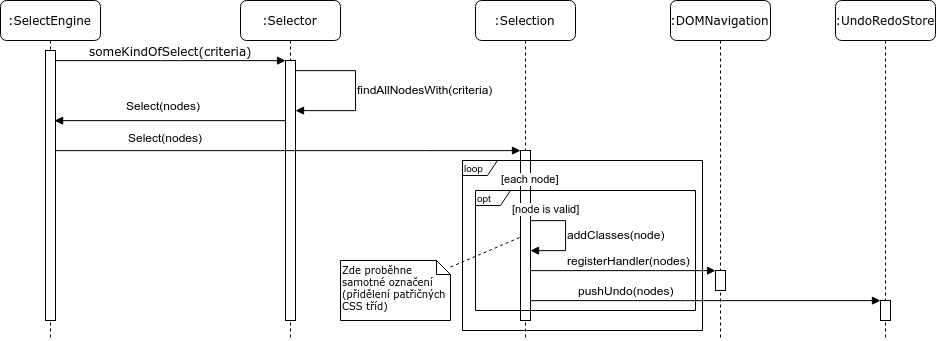
\includegraphics[width=\linewidth]{images/sequence_diagram.png}
	\caption{Sekvenční diagram naznačující průběh výběru dat}
	\label{fig:sequence_diagram}
\end{figure}

\subsection{Komunikace mezi třídami}
Jednotlivé třídy spolu interagují nepřímo, vždy přes rodičovskou komponentu (například třída TextSelector potřebuje volat metodu z třídy Selection, děje se tak ale přes rodičovskou třídu SelectEngine, viz diagram \ref{fig:sequence_diagram}). Důsledek tohoto faktu je patrný z diagramu \ref{fig:content_scripts_diagram}, který zobrazuje veškeré třídy reprezentující komponentu content script, kde se nachází téměř veškeré logika. Graf tříd tvoří stromovou strukturu a nikde nevznikají žádné cyklické závislosti. Díky tomu je dosaženo slabé provázanosti, jednoduché nahraditelnosti libovolné třídy a snadné rozšiřitelnosti.

\begin{figure}
	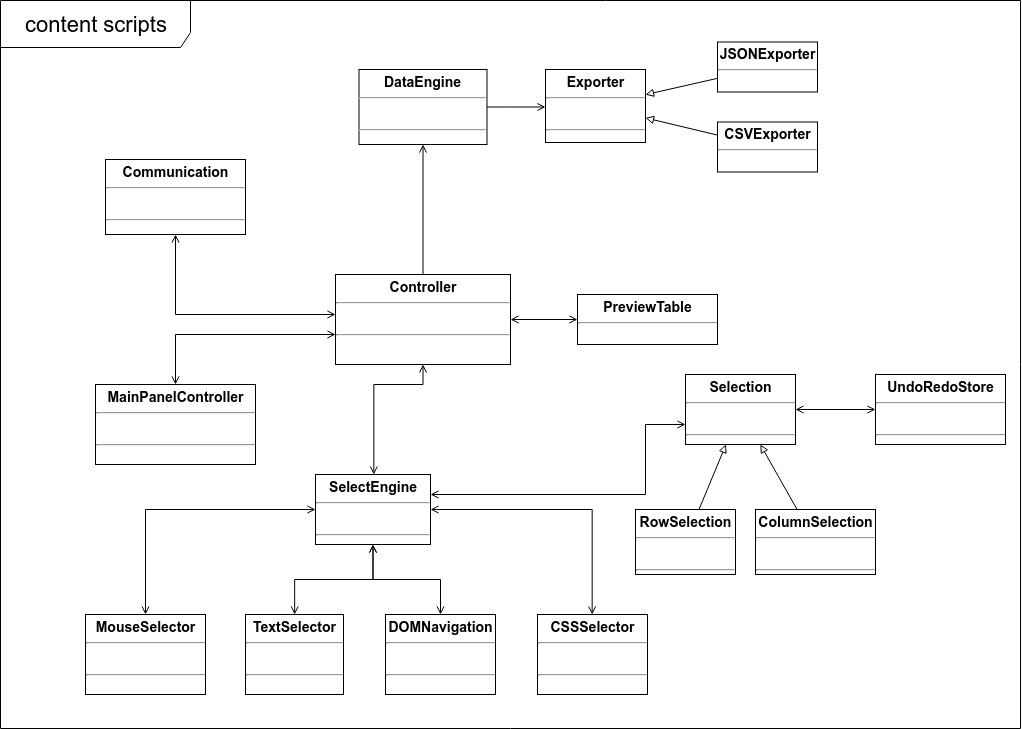
\includegraphics[width=\linewidth]{images/content_scripts_class_diagram.png}
	\caption[Diagram tříd reprezentujících komponentu content script]{Diagram tříd reprezentujících komponentu content script (pro přehlednost celého diagramu jsou uvedeny u každé třídy pouze ty nejdůležitější atributy a metody)}
	\label{fig:content_scripts_diagram}
\end{figure}

Tento postup však není možný v případě třídy MainPanel reprezentující ovládací panel vložený do stránky skrze iframe. Panelu není jak předat Controller, neboť to z bezpečnostních důvodů lze pouze v situaci, kdy je iframe i stránka, v níž je vložený, ze stejné domény\footnote{Opět narážíme na tzv. \emph{same-origin policy}.}. A to v tomto případě nejsou -- HTML stránka reprezentující ovládací panel pochází z domény rozšíření \verb|chrome-extension://<extension-id>|. 

Třídy MainPanel a Controller tak spolu komunikují skrze zasílání zpráv pomocí funkce \verb|window.postMessage()|, na které reaguje třída Communica-tion, jež je součástí hlavního Controlleru. Tato třída taktéž zajišťuje komunikaci mezi background scriptem a Controllerem. Diagram ... pak právě tuto komunikaci ilustruje.

\subsection{Extrakce dat}
Návrh aplikace pouze říká, že extrakce dat proběhne v prohlížeči na straně klienta a konkrétním implementacím ponechává volnost v řešení tohoto problému. Jelikož je nutné již vybrané prvky zvýraznit, přidává se ke každému takovému elementu příslušná CSS třída. Toho lze velmi jednoduše využít i při samotné extrakci dat -- aplikace nejdříve načte všechny elementy s třídou reprezentující řádky výsledné tabulky a v každém tomto elementu posléze načte všechny dostupné prvky s třídou reprezentující sloupce, z nichž vyextrahuje text (HTML atribut \textsf{innerText}), případně zdroj (HTML atribut \textsf{src}) v případě obrázků. To vše opět s pomocí funkce \verb|document.querySelectorAll()|, díky čemuž se jedná o velmi rychlý a efektivní způsob extrakce dat bez nutnosti zasílání požadavků na vzdálený server a je tak splněn nefunkční požadavek na rychlost samotné extrakce dat (N6).

Výsledná data jsou uložena v třídě DataEngine do doby, než je provedena operace, jež je nějakým způsobem ovlivňuje -- výběr nového prvku, zrušení stávajícího výběru, vytvoření nového sloupce, zrušení stávajícího sloupce. Poté se extrakce opakuje nanovo.
\clearpage
Na závěr jsou data převedena do požadovaného formátu pomocí třídy Exporter a je vytvořena URL adresa souboru. Ta se zašle background scriptu, který se už postará o samotné stažení -- otevře dialog vyzývající uživatele k vybrání umístění souboru.

\subsection{Ostatní}
?

% ================================================================================================
% Návod na instalaci extensionu, spuštění testů --- asi až v README

\chapter{Testování}
K testování celého kódu je použit JavaScriptový testovací framework Jest. Testy jsou rozděleny do dvou kategorií, a sice jednotkové (unit) testy a integrační testy, které víceméně simulují běžné používání nástroje. V posledních dvou sekcích se pak věnuji zhodnocení zadaných požadavků a nedostatkům, na něž by uživatelé mohli narazit.

% ------------------------------------------------------------------------------------------------

\section{Unit testy}
Jednotkové testy prověřují funkčnost každé třídy/funkce zvlášť, nezávisle na ostatních částech aplikace. K tomu je hojně využívána technika zvána \emph{mocking} -- závislosti testované třídy jsou místo reálných objektů splněny tzv. \emph{mocky}, které velmi zjednodušeně simulují chování zastupovaného objektu. Často se děje, že testovaná funkce potřebuje volat metody na objektu, jenž je do třídy dodán při jeho vytvoření. Místo použití reálného objektu tak stačí vytvořit objekt, který poskytuje stejné rozhraní (metody a atributy) a vrací pouze napevno dané hodnoty, což nám při testovaní většinou postačí.

Framework Jest pak velmi ulehčuje práci s těmito \emph{mockovanými} funkcemi. Umožňuje testovat, kolikrát byla daná funkce zavolána, s jakými parametry, jaká byla návratová hodnota apod. Jako příklad můžeme uvést funkci \verb|undo()| z třídy Selection -- ta pouze deleguje žádost zavoláním stejnojmenné metody na instanci třídy UndoRedoStore. Jeden ze způsobů testování pak ilustruje ukázka kódu \ref{code:mocking}, kdy pouze kontrolujeme, že byla patřičná funkce zavolána (jak je vidět z implementace na řádku 2, \emph{mockovaná} funkce často nemusí ani nic dělat).

Součástí frameworku Jest je také knihovna JSDOM, která hraje velmi důležitou roli při testování vyvíjeného nástroje. Jelikož se většina funkcionality aplikace týká manipulace se stránkou (jejím DOMem), je tato knihovna nezbytná -- implementuje totiž webové standardy, hlavně pak DOM a HTML, čímž do jisté míry simuluje webový prohlížeč a je tak ideálním nástrojem k testování aplikace. Nutno ale podotknout, že knihovna JSDOM nevykonává žádný rendering a layouting stránky, tedy jednotlivé elementy nejsou nikde zobrazené a jedná se opravdu jen o simulaci. S tím je spojená absence určitých atributů a funkcí, na něž jsme normálně zvyklí z klasických prohlížečů -- jmenovitě například atributy \textsf{offestWidth} a \textsf{offsetHeight}, které jsou v aplikaci kontrolovány při každém označování elementů (viz sekce \ref{sec:data_selection} Výběr dat). Tyto atributy jsou pak dodatečně definovány před spuštěním jednotlivých testů pomocí metody \verb|Object.defineProperty()|, viz ukázka kódu \ref{code:setup}.

\begin{figure}
	\begin{lstlisting}[language=JavaScript]
class UndoRedoStoreMockup {
	undo = jest.fn(() => {});
}
	
test('undo is called', () => {
	const undoRedoStore = new UndoRedoStoreMockup();
	const rowSelection = new RowSelection();
	rowSelection._undoRedoStore = undoRedoStore;
	
	expect(undoRedoStore.undo.mock.calls.length).toBe(0);
	rowSelection.undo();
	expect(undoRedoStore.undo.mock.calls.length).toBe(1);
});
	\end{lstlisting}
	\caption{Testovací přístup zvaný \emph{mocking}}
	\label{code:mocking}
\end{figure}

\begin{figure}
	\begin{lstlisting}[language=JavaScript]
// Mocking the `offsetWidth` HTML property
const target = targetWindow.HTMLElement.prototype;
const property = 'offsetWidth';
const getter = () => {
	return this._customOffsetWidth !== undefined 
		? this._customOffsetWidth 
		: 123;
};

Object.defineProperty(target, property, { get: getter });
	\end{lstlisting}
	\caption{Způsob definování HTML atributů}
	\label{code:setup}
\end{figure}


% ------------------------------------------------------------------------------------------------

\section{Integrační testy}
Zatímco jednotkové testy ověřují funkčnost jednotlivých tříd izolovaně od ostatních, integrační testy mají za úkol prověřit jejich korektní funkci při spolupráci celého systému. Jsou tak velmi užitečné k odhalování chyb při komunikaci mezi různými komponentami nebo předávání parametrů. V těchto testech tedy není využita technika \textit{mockování} -- výjimkou je celé Chrome API, které poskytuje právě prohlížeč Google Chrome. To samozřejmě při testování dostupné není, je tak nutné zařídit dostupnost funkcí, jež jsou v kódu volány. Z tohoto důvodu není vůbec testována funkcionalita komponenty background script, neboť bychom ověřovali pouze \textit{mockované} funkce.

Všechny integrační testy mají podobný průběh a cílí především na co nejvěrnější simulaci reálného používání. Na začátku je vytvořena instance třídy JSDOM, která načte testovací HTML stránku. Zpřístupní se tak klasické globální proměnné jako \verb|window|, \verb|window.document| a jejich metody jako \verb|document.querySelector()| nebo \verb|document.createElement()|. Poté je vytvořena a inicializována instance třídy Controller, jež je za normálních pod-mínek zavedena prohlížečem (pomocí komponenty \hyperref[def:content_script]{content script}, viz sekce \ref{sec:used_technology} Použité technologie). Po tomto kroku je celé rozšíření připravené k testování a chová se téměř stejně jako v obyčejném prohlížeči.

Jedním z problému, jež nastaly při testování, byl fakt, že JSDOM nepodporuje skripty využívající moduly, resp. syntaxi ES6 (\verb|import| a \verb|export|). Avšak všechen kód je psaný právě s touto syntaxí a vkládán do HTML stránky pomocí \verb|<script type="module"></script>|. Řešením tak je načtení všech skriptů, jež jsou načítány tímto způsobem, do paměti, smazání problematických klíčových slov a vytvoření jediného skriptu, který obsahuje všechen potřebný kód.

V neposlední řadě pak integrační testy také simulují všechny popsané případy užití v sekci \ref{sec:use_cases} Případy užití a demonstrují běžné zacházení s nástro-jem, jako je možné vidět v ukázce kódu \ref{code:integration_test}.

\begin{figure}
	\begin{lstlisting}[language=JavaScript]
	import { startMouseSelection } from './integrationUtils.js';
	import { _click, _clickWithCtrl } from '../utils.js';
	
	function isSelected(node, id) {
		const c1 = node.classList.contains('scraping-selected-row');
		const c2 = node.classList.contains(`scraping-row-${id}`);
		expect(c1).toBe(true);
		expect(c2).toBe(true);
	}
	
	test('use case #1', async () => {
		const selector = 'tr:not(.scraping-protected)';
		const rows = document.querySelectorAll(selector);
		const firstRow = allTableRows[0];
		const secondRow = allTableRows[1];
		
		await startMouseSelection(panelDocument);
		_click(firstRow);
		isSelected(firstRow, 0);
	
		_clickWithCtrl(secondRow);
		isSelected(secondRow, 0);
	
		for (let i = 0; i < rows.length; i++) {
			isSelected(rows[i], i);
		}
	});
	\end{lstlisting}
	\caption{Způsob definování HTML atributů}
	\label{code:integration_test}
\end{figure}

% ------------------------------------------------------------------------------------------------

\section{Naplnění zadaných požadavků}
Součástí každého projektu by mělo být také zhodnocení předsevzatých cílů, především pak splnění všech definovaných požadavků na vyvíjený software. Těmi hlavními byly:

\begin{itemize}
	\item Aplikace umožňující extrahovat data z webových stránek uživatelům neznalých programování -- to jest splněno, neboť primární způsob užití nástroje je založen na visual scrapingu (označování prvků myší na strán-ce) nebo textovém vyhledávání a nevyžaduje od uživatelů žádné znalosti z oblasti IT.
	\item Jednoduché a intuitivní ovládání, přehledné grafické rozhraní, jenž nebude zahlcené přebytkem možností -- v porovnání s ostatními nástroji je užívání vyvinuté aplikace velmi rychlé a počet kroků požadovaných od uživatele minimální. To je z velké míry docíleno úzkým zaměřením nástroje. 
	\item Snadná rozšiřitelnost pro přidávání další funkcionality -- viz kapitoly Návrh a Realizace.
\end{itemize}

Všechny tyto požadavky byly úspěšně splněny a výsledkem je funkční nástroj, připravený k použití. Tím, že se jedná o rozšíření do internetového prohlížeče Google Chrome, v podstatě odpadá fáze nasazení -- výslednou aplikaci stačí publikovat v internetovém obchodě Chrome (Chrome Web Store).\footnote{To se reálně v rámci této práce nestalo, neboť před prvním zveřejněním libovolného rozšíření je nutné zaplatit jednorázový poplatek.}

Zároveň nebyly dotaženy do konce všechny zadané požadavky. Požadavek F9) říká, že data půjdou exportovat do tří formátů -- JSON, CSV a XLS. To bylo splněno pouze částečně, neboť XLS formát (používaný programem Microsoft Excel) se ukázal jako zbytečně složitý na implementaci a zároveň nepřináší v rámci vyvíjené aplikace žádné benefity. Microsoft Excel podporuje i soubory formátu CSV a jelikož jsou exportovaná data vždy pouze tabulkou s textovými hodnotami, nemá formát XLS smysl (žádné funkce, grafy, makra ani jiné podobné výhody tohoto formátu nejsou využity). V průběhu vývoje od něj tedy bylo nakonec upuštěno a byly implementovány pouze formáty JSON a CSV.

Naopak byl splněn požadavek +2) na přesouvání a minimalizaci ovládacího panelu. Pro úplnost je pak uvedena tabulka \ref{table:requirements} se všemi požadavky a přehled jejich naplnění (zelená barva značí kompletní splnění, žlutá částečně splnění a červená nesplnění požadavku).

\begin{table}
	\centering
	\caption{Přehled naplnění jednotlivých požadavků}
	\label{table:requirements}
	\begin{tabular}{ | c | c | }
		\hline
		Kód & Požadavek \\
		\hline
		\rowcolor{lightgreen}
		F1 & UI se skládá z pracovní plochy a ovládacího panelu \\
		\rowcolor{lightgreen}
		F2 & Ovládací panel je rozdělen do záložek \\
		\rowcolor{lightgreen}
		F3 & Extrakce textu z elementů \\
		\rowcolor{lightgreen}
		F3.1 & Výběr pomocí myši \\
		\rowcolor{lightgreen}
		F3.2 & Výběr pomocí textového vyhledávání \\
		\rowcolor{lightgreen}
		F3.3 & Výběr pomocí CSS selektorů \\
		\rowcolor{lightgreen}
		F3.4 & Navigace výběru napříč DOMem \\
		\rowcolor{lightred}
		F3.5 & Šablony akcí \\
		\rowcolor{lightgreen}
		F4 & Extrakce atributu \textsf{src} z img tagů \\
		\rowcolor{lightgreen}
		F5 & Auto-selection \\
		\rowcolor{lightgreen}
		F6 & Undo a redo \\
		\rowcolor{lightgreen}
		F7 & Označení již vybraných elementů \\
		\rowcolor{lightgreen}
		F8 & Preview mód \\
		\rowcolor{lightyellow}
		F9 & Export do JSON, CSV, XLS \\
		\hline
		\rowcolor{lightred}
		N1 & Webová aplikace bez nutnosti instalace \\
		\rowcolor{lightgreen}
		N2 & Pouze frontend \\
		\rowcolor{lightgreen}
		N3 & Přehledné GUI, přímočaré ovládání \\
		\rowcolor{lightgreen}
		N4 & Snadná rozšiřitelnost aplikace \\
		\rowcolor{lightgreen}
		N5 & Co nejkratší doba strávená výběrem dat \\
		\rowcolor{lightgreen}
		N6 & Čas extrakce dat nepřesáhne 5 vteřin \\
		\hline
		\rowcolor{lightred}
		+1 & Klávesové zkratky \\
		\rowcolor{lightgreen}
		+2 & Přesouvání a minimalizace ovládacího panelu \\
		\rowcolor{lightred}
		+3 & Další možnosti exportu \\
		\rowcolor{lightred}
		+4 & Interaktivní tutoriál \\
		\rowcolor{lightred}
		+5 & Tvorba filtru na základě výběru \\
		\hline
	\end{tabular}
\end{table}

% ------------------------------------------------------------------------------------------------

\section{Nedostatky aplikace}
Za hlavní nedostatek nástroje považuji chybějící web crawling, kvůli čemuž je aplikace vhodná pouze na statické extrahování dat z jedné stránky. Na druhou stranu je takto vymezená již od začátku a právě díky absenci této funkcionality je její ovládaní velice jednoduché a přímočaré.

Tím, že se jedná o rozšíření do internetové prohlížeče Google Chrome, nemá uživatel na výběr a musí (alespoň po dobu využívání nástroje) používat právě tento prohlížeč. V tom spatřuji další nedostatek, neboť by pro někoho mohlo jít o překážku. Tento problém má ale částečné řešení -- dle \cite{extension_porting} mají prohlížeče Chrome, Firefox a Opera téměř stejné API, které jejich rozšíření používají. Tím pádem je možné rozšíření psané primárně pro prohlížeč Chrome s minimální námahou převést na rozšíření pro prohlížeče Firefox a Opera.

% ================================================================================================

\begin{conclusion}
	V~bakalářské práci jsem se zabýval analýzou web scrapingu a především pak právní problematikou, jež představuje první ze dvou vedlejších cílů. Uvedl jsem základní pojmy a zasadil web scraping do kontextu českého právního systému. Také jsem představil nejvýznamnější soudní případy zabývající se právě vytě-žováním dat z~internetových stránek, díky kterým jsme se mohli přesvědčit, že zatím neexistuje jednotné stanovisko při určování, co je v~rozporu s~právem a co ne. V~nejbližší budoucnosti však můžeme být svědky formování a zrodu jednotného precedentu, dle něhož se soudy mohou řídit. Užitek bakalářské práce pak spatřuji hlavně v~tomto právním souhrnu, který může posloužit jako dobrý úvod do hlubšího pátrání.
	
	Poté jsem se věnoval druhému z~vedlejších cílů, a sice rešerši stávajících řešení. Nástrojů poskytujících uživatelské rozhraní pro vytěžování dat z~webo-vých stránek existuje nespočet, avšak téměř všechny se snaží nabídnout co nejvíce funkcionalit a možností na úkor uživatelského zážitku a jednoduchosti používání. Přesně tomu se snaží vyhnout software vyvinutý v~rámci této práce, čímž přecházím k~hlavnímu cíli -- vývoji samotného softwaru.
	
	V~rané fázi vývoje nastaly neočekávané komplikace. Implementace návrhu jakožto webové aplikace najednou nepřipadala v~úvahu kvůli HTTP hlavičce omezující možnost zabudovat libovolný HTML dokument uvnitř své vlastní stránky. Musel jsem tedy upustit od svého původního záměru a najít lepší řešení. Tím je implementace v~podobě rozšíření do internetového prohlížeče, které je dle mého názoru elegantním řešením daného problému.
	
	Jak již bylo několikrát řečeno, přínos samotné aplikace spočívá především v~její jednoduchosti. Z~toho mohou těžit uživatelé, kteří se nezabývají programováním nebo tvorbou webových stránek. Využije ji tak kdokoli, kdo potřebuje jednorázově získat data z~webové stránky, jež obsahuje velké množ-ství dat pohromadě na jedno místě. Z~důvodu chybějící automatizace a crawlingu je naopak nevhodná k~pravidelnému získávání dat (jako je například dlouhodobé sledování cen produktů) či ke zpracování stránek, kde se jednotlivá data nacházejí rozptýlená po celé doméně.
	
	Hlavní i~vedlejší cíle tak považuji za úspěšně splněné. Zároveň se zde otevírá obrovský prostor pro potenciální navazující práce. Na tomto základu by mohla vzniknout opravdu hluboká a plnohodnotná právní analýza celé domény. Taktéž nástroj samotný je díky splnění požadavku na snadnou rozšiři-telnost připraven pro další vylepšení, ať už by se jednalo o~dokončení všech definovaných požadavků (z kategorie \textit{nice-to-have}) či přidání klíčové funkcionality, která by diametrálně změnila jeho konkurenceschopnost -- web crawlingu nebo možnosti automatizace.
\end{conclusion}

% ================================================================================================

\begin{thebibliography}{99}
	\bibitem{web_scraping_def}
	VARGIU, Eloisa; URRU, Mirko. Exploiting web scraping in a collaborative filtering-based approach to web advertising. \textit{Artificial Intelligence Research} [online]. 2013, roč. 2, č. 1 [cit. 13. 4. 2019]. DOI: 10.5430/air.v2n1p44. ISSN 1927-6974. Dostupné z: \url{http://www.sciedu.ca/journal/index.php/air/article/view/1390/1115}.
	
	\bibitem{web_crawler_def}
	KOBAYASHI, Mei; TAKEDA, Koichi. Information Retrieval on the Web. \textit{ACM Computing Surveys} [online]. 2000, roč. 32, č. 2 [cit. 13. 4. 2019]. DOI: 10.1145/358923.358934. ISSN 0360-0300. Dostupné z: \url{https://dl.acm.org/citation.cfm?doid=358923.358934}.
	
	\bibitem{web_wanderer}
	World Wide Web Wanderer. In: \textit{History-Computer} [online] [cit 13. 4. 2019]. Dostupné z: \url{https://history-computer.com/Internet/Conquering/Wanderer.html}.
	
	\bibitem{web_scraping_history}
	Web Scraping: How It All Started And Will Be. In: \textit{Octoparse's blog} [online]. © 2019 Octopus Data Inc. [cit. 13. 4. 2019]. Dostupné z: \url{https://www.octoparse.com/blog/web-scraping-introduction}.
	
	\bibitem{computer_vision}
	ROUSH, Wade. Diffbot Is Using Computer Vision to Reinvent the Semantic Web. In: \textit{Xconomy} [online]. © 2007--2019, Xconomy [cit. 13. 4. 2019]. Dostupné z: \url{https://xconomy.com/san-francisco/2012/07/25/diffbot-is-using-computer-vision-to-reinvent-the-semantic-web/}.
	
	\bibitem{data_size}
	WASSÉN, Olivia. Big Data facts -- How much data is out there? In: \textit{NodeGraph} [online]. © 2019 NodeGraph [cit. 13. 4. 2019]. Dostupné z: \url{https://www.nodegraph.se/big-data-facts/}.
	
	\bibitem{google_bot}
	Googlebot. In: \textit{Google Help Center} [online]. © 2019 Google [cit 23. 4. 2019]. Dostupné z: \url{https://support.google.com/webmasters/answer/182072}.
	
	\bibitem{data_mining}
	CLIFTON, Christopher. Data mining. In: \textit{Encyclopædia Britannica} [online]. ©2019 Encyclopædia Britannica, Inc. [cit. 13. 4. 2019]. Dostupné z: \url{https://www.britannica.com/technology/data-mining}.
	
	\bibitem{browse_wrap}
	KUNKEL, R. G. Recent developments in shrinkwrap, clickwrap and browsewrap licenses in the United States. \textit{MurUEJL} [online]. 2002, roč. 9, č. 3 [cit. 1. 4. 2019]. Dostupné z: \url{http://www5.austlii.edu.au/au/journals/MurUEJL/2002/34.html}.
	
	\bibitem{take_it_or_leave_it}
	What Is a Take It or Leave It Contract? In: \textit{UpCounsel} [online]. © 2019 UpCounsel, Inc. [cit. 1. 4. 2019]. Dostupné z: \url{https://www.upcounsel.com/take-it-or-leave-it-contract}.
	
	\bibitem{click_wrap}
	OBAR, Jonathan A.; OELDORF-HIRSCH, Anne. The Clickwrap: A~Political Economic Mechanism for Manufacturing Consent on Social Media. \textit{Social Media + Society} [online]. 2018, roč. 4, č. 3 [cit. 1. 4. 2019]. DOI: 10.1177/2056305118784770. ISSN 2056-3051. Dostupné z: \url{https://journals.sagepub.com/doi/10.1177/2056305118784770}.
	
	\bibitem{rozhovor}
	VAŠÍČEK, Libor. [osobní sdělení]. Advokát specializující se na ICT právo a autorské právo. Sídlo advokátní kanceláře Legal Partners, s.~r.~o., Záhořanského 1944/4, Praha 2. 29. března 2019.
	
	\bibitem{obcansky_zakon}
	ČESKO. Zákon č. 89/2012 Sb, občanský zákoník. In: \textit{Zákony pro lidi.cz} [online]. © AION CS 2010--2019 [cit. 30. 3. 2019]. Dostupné z: \url{https://www.zakonyprolidi.cz/cs/2012-89}.
	
	\bibitem{autorsky_zakon}
	ČESKO. Zákon č. 121/2000 Sb., o~právu autorském, o~právech souvisejících s~právem autorským a o~změně některých zákonů (autorský zákon). In: \textit{Zákony pro lidi.cz} [online]. © AION CS 2010--2019 [cit.~30.~3.~2019]. Dostupné z: \url{https://www.zakonyprolidi.cz/cs/2000-121}.
	
	\bibitem{polcak}
	POLČÁK, Radim. \textit{Právo informačních technologií}. Praha: Wolters Kluwer, 2018. Právní monografie (Wolters Kluwer ČR). 656 stran. ISBN 978-80-7598-045-8.
	
	\bibitem{ikaros}
	SMEJKAL, Ladislav. Právní ochrana databází v~novém autorském zákoně. \textit{Ikaros} [online]. 2001, roč. 5, č. 3 [cit. 13. 4. 2019]. urn:nbn:cz:ik-10688. ISSN 1212-5075. Dostupné z: \url{http://ikaros.cz/node/10688}.
	
	\bibitem{C-444/02_1}
	Věc C-444/02, stanovisko generální advokátky ze dne 8. června 2004 ve věci Fixtures Marketing Ltd v. Organismos prognostikon agonon podosfairou AE (OPAP). In: \textit{EUR-Lex} [online]. © European Union, 1998--2019 [cit. 30. 3. 2019]. Dostupné z: \url{https://eur-lex.europa.eu/legal-content/CS/TXT/?uri=CELEX:62002CC0444}.
	
	\bibitem{C-444/02_2}
	Věc C-444/02, rozsudek Soudního dvora (velkého senátu) ze dne 9. listopadu 2004 ve věci Fixtures Marketing Ltd v. Organismos prognostikon agonon podosfairou AE (OPAP). In: \textit{EUR-Lex} [online]. © European Union, 1998--2019 [cit. 30. 3. 2019]. Dostupné z: \url{https://eur-lex.europa.eu/legal-content/CS/TXT/?uri=CELEX:62002CJ0444}.
	
	\bibitem{C-30/14}
	Věc C-30/14, rozsudek Soudního dvora (druhého senátu) ze dne 15. ledna 2015 ve věci Ryanair Ltd v. PR Aviation BV. In: \textit{EUR-Lex} [online]. © European Union, 1998--2019 [cit. 30. 3. 2019]. Dostupné z: \url{https://eur-lex.europa.eu/legal-content/CS/TXT/?uri=CELEX:62014CJ0030}.
	
	\bibitem{hiq_linkedin_1}
	Case 17-cv-03301-EMC, order granting plaintiff's motion for preliminary injunction, filed 08/14/17. In: \textit{The United States District Court for the Northern District of California} [online]. United States District Court [cit. 30. 3. 2019]. Dostupné z: \url{https://www.cand.uscourts.gov/filelibrary/3170/C-17-3301-hiQ-v.-LinkedIn-Order-Docket-No.-63.pdf}.
	
	\bibitem{linkedin_arg}
	WILLIAMS, Jamie. ‘Scraping’ Is Just Automated Access, and Everyone Does It. In: \textit{Electronic Frontier Foundation} [online]. Electronic Frontier Foundation [cit. 1. 4. 2019]. Dostupné z: \url{https://www.eff.org/deeplinks/2018/04/scraping-just-automated-access-and-everyone-does-it}
	
	\bibitem{public_forum}
	Forums. In: \textit{Legal Information Institute} [online]. Cornell Law School [cit. 30. 3. 2019]. Dostupné z: \url{https://www.law.cornell.edu/wex/forums}.
	
	\bibitem{hiq_linkedin_2}
	NARULA, Prayag. LinkedIn Vs. hiQ Ruling Casts A~Long Shadow Over The Tech Industry. In: \textit{Forbes} [online]. © 2019 Forbes Media LLC [cit. 30. 3. 2019]. Dostupné z: \url{https://www.forbes.com/sites/forbestechcouncil/2017/09/20/linkedin-vs-hiq-ruling-casts-a-long-shadow-over-the-tech-industry}.
	
	\bibitem{facebook_venture_1}
	Case 13-17154, Facebook v. Vachani. In: \textit{United States Court of Appeals for the Ninth Circuit} [online]. [cit. 31. 3. 2019]. Dostupné z: \url{https://cdn.ca9.uscourts.gov/datastore/opinions/2016/07/12/13-17102.pdf}.
	
	\bibitem{facebook_venture_2}
	KERR, Orin. 9th Circuit: It’s a federal crime to visit a website after being told not to visit it. In: \textit{The Washington Post} [online]. © 1996--2019 The Washington Post [cit. 31. 3. 2019]. Dostupné z: \url{https://www.washingtonpost.com/news/volokh-conspiracy/wp/2016/07/12/9th-circuit-its-a-federal-crime-to-visit-a-website-after-being-told-not-to-visit-it}.
	
	\bibitem{content_grabber}
	Stránka. \textit{Content Grabber} [online] [cit. 26. 4. 2019]. Dostupné z: \url{http://www.contentgrabber.com}.
	
	\bibitem{mozenda}
	Stránka. \textit{Mozenda} [online] [cit. 26. 4. 2019]. Dostupné z \url{https://www.mozenda.com}.
	
	\bibitem{parsehub}
	PARSEHUB. \textit{ParseHub. Version 54.0.1} [software]. 2015 [cit. 13. 4. 2019]. Dostupné z: \url{https://www.parsehub.com/quickstart}.
	
	\bibitem{octoparse}
	OCTOPUS DATA INC. \textit{Octoparse. Version 7.1.2} [software]. 2018 [cit. 13. 4. 2019]. Dostupné z: \url{https://www.octoparse.com/download}.
	
	\bibitem{webscraper}
	WEBSCRAPER. \textit{WebScraper. Version 0.3.8.9} [software]. 2016 [cit. 13. 4. 2019]. Dostupné z: \url{https://chrome.google.com/webstore/detail/web-scraper/jnhgnonknehpejjnehehllkliplmbmhn}.
	
	\bibitem{dexio}
	DEXI APS. \textit{Dexi.io} [software] [cit. 13. 4. 2019]. Dostupné z: \url{https://app.dexi.io/}.
	
	\bibitem{data_scraper}
	SOFTWARE INNOVATION LAB LLC. \textit{Data scraper. Version 3.299.84} [software]. 2015 [cit. 13. 4. 2019]. Dostupné z: \url{https://chrome.google.com/webstore/detail/data-scraper-easy-web-scr/nndknepjnldbdbepjfgmncbggmopgden}.
	
	\bibitem{iframe}
	\textless iframe\textgreater: The Inline Frame element. In: \textit{MDN web docs} [online]. © 2005--2019 Mozilla [cit. 4. 5. 2019]. Dostupné z: \url{https://developer.mozilla.org/en-US/docs/Web/HTML/Element/iframe}.
	
	\bibitem{x_frame_options}
	X-Frame-Options. In: \textit{MDN web docs} [online]. © 2005--2019 Mozilla [cit. 4. 5. 2019]. Dostupné z: \url{https://developer.mozilla.org/en-US/docs/Web/HTTP/Headers/X-Frame-Options}.
	
	\bibitem{clickjacking}
	Clickjacking. In: \textit{Imperva} [online]. © 2019 Imperva [cit. 4. 5. 2019]. Dostupné z: \url{https://www.imperva.com/learn/application-security/clickjacking/}.
	
	\bibitem{clickjacking_defense}
	Law, Eric. Combating ClickJacking With X-Frame-Options. In: \textit{MSDN Blogs} [online]. © 2019 Microsoft [cit. 4. 5. 2019]. Dostupné z: \url{https://blogs.msdn.microsoft.com/ieinternals/2010/03/30/combating-clickjacking-with-x-frame-options/}.
	
	\bibitem{extension_porting}
	Porting a Google Chrome extension. In: \textit{MDN web docs} [online]. © 2005--2019 Mozilla [cit. 2. 5. 2019]. Dostupné z: \url{https://developer.mozilla.org/en-US/docs/Mozilla/Add-ons/WebExtensions/Porting_a_Google_Chrome_extension}.
	
\end{thebibliography}

\appendix


% ================================================================================================


\chapter{Seznam použitých zkratek}
% \printglossaries
\begin{description}
	\item[API] Application Programming Interface
	\item[CAN-SPAM] Controlling the Assault of Non-Solicited Pornography and Marketing Act
	\item[CFAA] Computer Fraud and Abuse Act
	\item[CSS] Cascading Style Sheets
	\item[CSV] Comma-Separated Values
	\item[DOM] Document Object Model
	\item[HTML] HyperText Markup Language
	\item[IP] Internet Protocol
	\item[JSON] JavaScript Object Notation
	\item[MIT] Massachusetts Institute of Technology
	\item[URL] Uniform Resource Locator
	\item[XLS] formát souboru používaný aplikací Microsoft Excel
	\item[XML] eXtensible Markup Language
\end{description}

% ================================================================================================

\chapter{Obsah přiloženého CD}

%upravte podle skutecnosti

\begin{figure}
	\dirtree{%
		.1 readme.txt\DTcomment{stručný popis obsahu CD}.
		.1 exe\DTcomment{adresář se spustitelnou formou implementace}.
		.1 src.
		.2 impl\DTcomment{zdrojové kódy implementace}.
		.2 thesis\DTcomment{zdrojová forma práce ve formátu \LaTeX{}}.
		.1 text\DTcomment{text práce}.
		.2 thesis.pdf\DTcomment{text práce ve formátu PDF}.
		.2 thesis.ps\DTcomment{text práce ve formátu PS}.
	}
\end{figure}

\end{document}
